% Load the kaobook class
\documentclass[
	fontsize=10pt, % Base font size
	twoside=true, % Use different layouts for even and odd pages (in particular, if twoside=true, the margin column will be always on the outside)
	%open=any, % If twoside=true, uncomment this to force new chapters to start on any page, not only on right (odd) pages
%%	secnumdepth=1, % How deep to number headings. Defaults to 1 (sections)
]{kaobook}


\newcommand{\discipline}{Sciences Industrielles de l'Ingénieur }
\newcommand{\auteur}{Thomas Lusseau}
\newcommand{\repRel}{../}


\input{\repRel/Style/packages_v2}
\newcommand{\repStyle}{\repRel/Style}
\input{\repRel/Style/macros_SII_v2}
\input{\repRel/Style/environment_v2}
\usepackage{\repStyle/UPSTI_pedagogique}

%Bob
\usepackage[most]{tcolorbox}
\usepackage{graphicx}
\usepackage{xparse}

\definecolor{exoBlue}{RGB}{35,85,160}

\newtcolorbox{exercice}[2][]{
    enhanced,
    breakable,
    colback=white,
    colframe=exoBlue,
    boxrule=1pt,
    arc=1mm,
    title={#2},
    colbacktitle=exoBlue,
    coltitle=white,
    fonttitle=\bfseries\Large,
    attach boxed title to top left={
        xshift=0mm,
        yshift=-2mm
    },
    boxed title style={
        sharp corners,
        boxrule=0pt
    },
    left=4mm,
    right=4mm,
    top=4mm,
    bottom=4mm,
    #1
}

\newtcolorbox{bobbox}[1][]{
    enhanced,
    breakable,
    colback=orange!10,
    colframe=orange!90!black,
    boxrule=0.8pt,
    arc=1mm,
    left=4mm,
    right=4 mm,
    top=4mm,
    bottom=4mm,
    %fontupper=\bfseries,
    halign=center,
overlay unbroken={
  \node[
    anchor=south east,
    inner sep=0pt,
    xshift=10mm
  ] at (frame.south east)
  {
 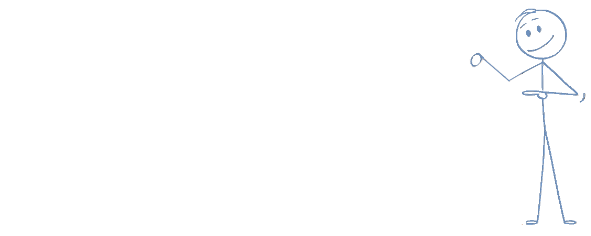
\includegraphics[height=3.2cm]{images/bob.png}
%    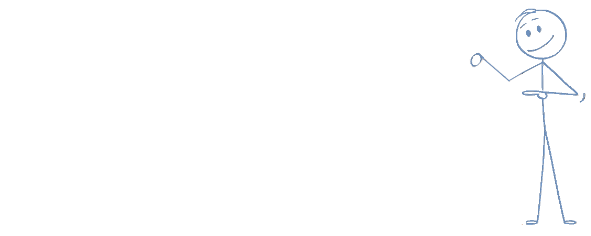
\includegraphics[
%height=\tcbtextheight\relax
%    ]{images/bob.png}
  };
},
    #1
}

\usepackage{tikz}
\usetikzlibrary{decorations.pathmorphing}

\definecolor{bobblue}{RGB}{45,78,120}



\NewDocumentEnvironment{bob}{O{}}
{\begin{bobbox}[#1]}
{\end{bobbox}}

% Choose the language
%\usepackage[english]{babel} % Load characters and hyphenation
%\usepackage[francais]{babel} % Load characters and hyphenation
\frenchsetup{StandardItemLabels=true}
%% \usepackage[english=british]{csquotes}	% English quotes

% Load packages for testing
%\usepackage{blindtext}
%\usepackage{showframe} % Uncomment to show boxes around the text area, margin, header and footer
%\usepackage{showlabels} % Uncomment to output the content of \label commands to the document where they are used

% Load the bibliography package
\usepackage{kaobiblio}
\addbibresource{Cy_01_ModelisationSystemes.bib} % Bibliography file

% Load mathematical packages for theorems and related environments
\usepackage{kaotheorems}

% Load the package for hyperreferences
\usepackage{kaorefs}

\usepackage[normalem]{ulem}
\providecommand{\ul}[1]{\uline{#1}}

\graphicspath{{images/}{./}} % Paths where images are looked for

\makeindex[columns=3, title=Alphabetical Index, intoc] % Make LaTeX produce the files required to compile the index


\usetikzlibrary{decorations.text,backgrounds,shadings}

\begin{document}

%%----------------------------------------------------------------------------------------
%%	BOOK INFORMATION
%%----------------------------------------------------------------------------------------

\titlehead{Thomas Lusseau - SII en ATS}
\title[Thomas Lusseau - SII en ATS]{Thomas Lusseau - SII en ATS}
\author[TL]{Thomas Lusseau}
\date{\today}


\begingroup % Local scope for the following commands
\setstretch{1} % Uncomment to modify line spacing in the ToC
%\tableofcontents % Output the table of contents
\endgroup

%%----------------------------------------------------------------------------------------
%%	MAIN BODY
%%----------------------------------------------------------------------------------------
%
\mainmatter % Denotes the start of the main document content, resets page numbering and uses arabic numbers
%\setchapterstyle{kao} % Choose the default chapter heading style
%
%\chapter{First Chapter}
%
%\blindtext
%
%\pagelayout{wide} % No margins
%\addpart{Title of the Part}
%\pagelayout{margin} % Restore margins
%
%\chapter{Second Chapter}

\setchapterstyle{kao}

\setcounter{margintocdepth}{\sectiontocdepth}
\marginlayout
\graphicspath{{\repStyle/png}}

\pagestyle{scrheadings}

\AtBeginEnvironment{corrige}{\small}

\livrettrue % Livrettrue :  eleve sans les corrections
%\livretfalse
\collefalse
%%%%%


% Conversion LaTeX du fichier Word "1-AnalyseFonctionnelle2022(1).docx"
% Images extraites dans le dossier ./images
% Fichier prévu pour être inclus dans votre projet kaobook / cours existant.
% Packages nécessaires dans le préambule principal : graphicx, xcolor, hyperref, longtable, booktabs, array, calc, multirow, ulem.

\graphicspath{{images/}}
\providecommand{\ul}[1]{\uline{#1}}

\setchapterimage{../Style/FondPoly.png}
\setchapterpreamble[u]{\margintoc}

\begingroup
\definecolor{kaoblue}{RGB}{0,82,155}
\addtokomafont{chapter}{\color{kaoblue}}
\chapter*{Introduction à l'ingénierie système}
\endgroup
\setcounter{chapter}{1}


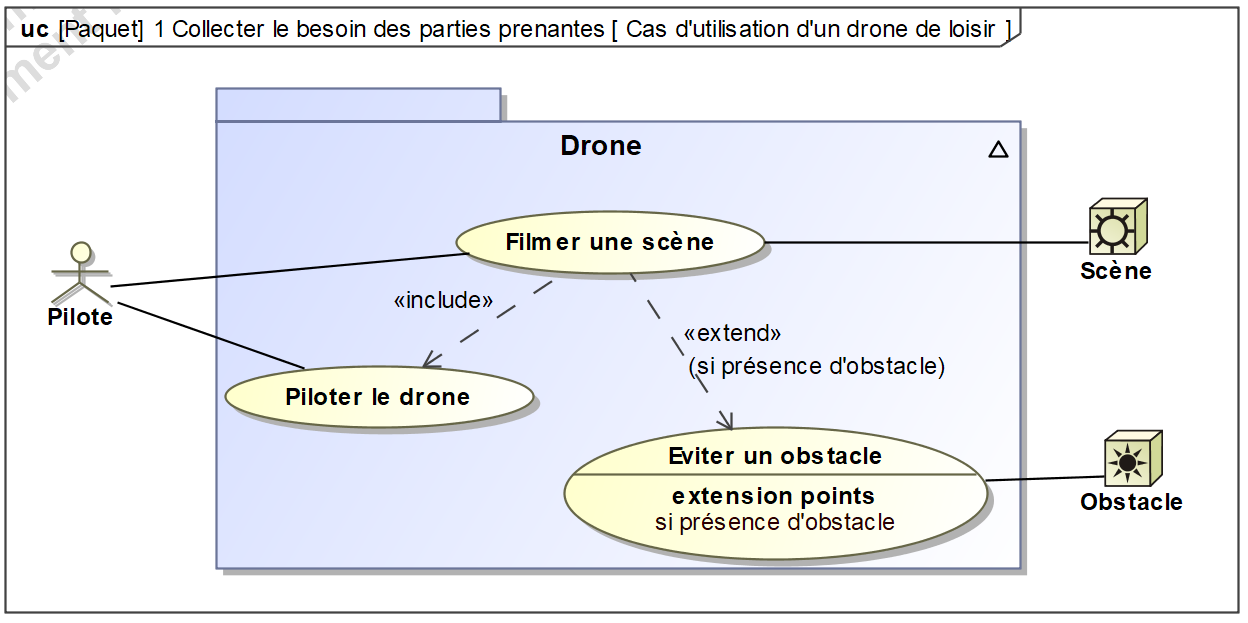
\includegraphics[width=\linewidth]{images/image3.png}

%\tableofcontents
\clearpage

\section{MISE EN SITUATION}\label{mise-en-situation}

\subsection{Cas n°1~: Repêchage d'une
voiture}\label{cas-n1-repuxeachage-dune-voiture}

Les photos suivantes illustrent\footnote{C\textquotesingle est
  l\textquotesingle illustration également du principe du bras de
  levier, et par là même une introduction aux actions mécaniques...} le
cas typique d\textquotesingle une situation où la solution envisagée ne
répond pas au besoin initial, ou n\textquotesingle est pas adaptée à
celui-ci. Cela s'est passé en septembre 2004, sur le quai de Roundstone
dans le Connemara, en Irlande.

\begin{longtable}[]{@{}
  >{\raggedright\arraybackslash}p{(\columnwidth - 2\tabcolsep) * \real{0.4998}}
  >{\raggedright\arraybackslash}p{(\columnwidth - 2\tabcolsep) * \real{0.5002}}@{}}
\toprule\noalign{}
\begin{minipage}[b]{\linewidth}\raggedright
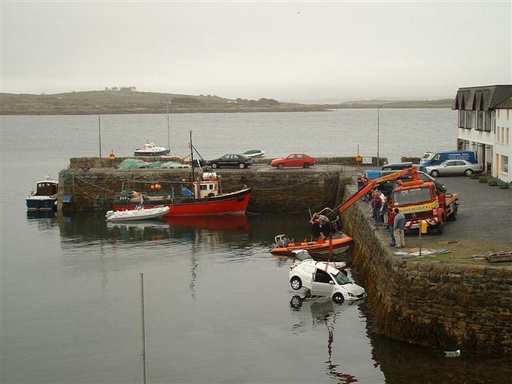
\includegraphics[width=\linewidth]{images/image5.jpeg}
\end{minipage} & \begin{minipage}[b]{\linewidth}\raggedright
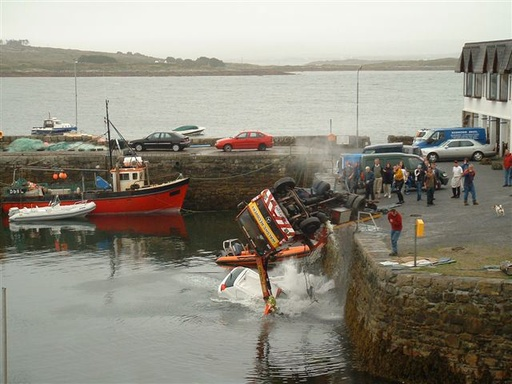
\includegraphics[width=\linewidth]{images/image6.jpeg}
\end{minipage} \\
\midrule\noalign{}
\endhead
\bottomrule\noalign{}
\endlastfoot
\emph{Un camion-grue repêche une voiture..} & \emph{... mais celle-ci
entraine le camion-grue.} \\
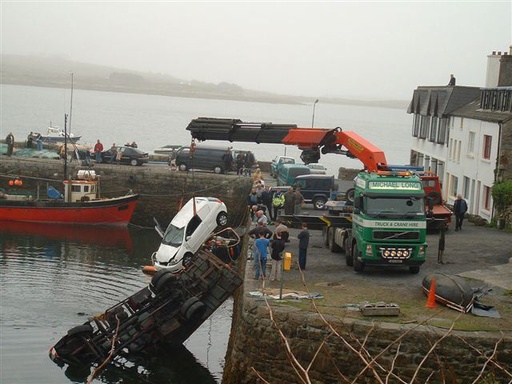
\includegraphics[width=\linewidth]{images/image7.jpeg}
&
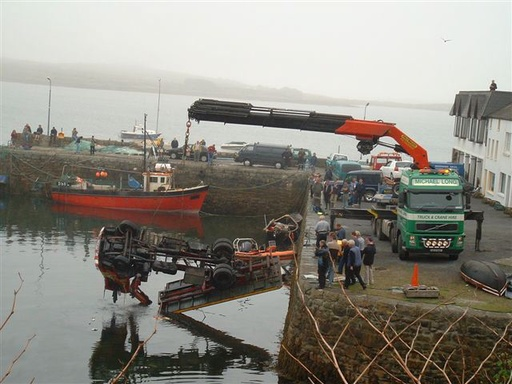
\includegraphics[width=\linewidth]{images/image8.jpeg} \\
\emph{Finalement un second camion-grue à stabilisateurs repêche la
voiture...} & \emph{... ainsi que le premier camion-grue.} \\
\end{longtable}

C\textquotesingle est le cas typique d\textquotesingle une solution dite
"de facilité", où pour des raisons budgétaires et/ou temporelles on
préfère user de solutions sous-optimales (en termes
d\textquotesingle efficacité, de fonctionnalités offertes), et qui bien
souvent engendrent des surcoûts ou des délais supplémentaires (soit donc
l\textquotesingle effet inverse de celui escompté).

\subsection{Cas n°2~: Trains}\label{cas-n2-trains}

En 2014, les nouveaux trains régionaux sont conçus plus larges que leurs
prédécesseurs, afin de répondre au mieux aux attentes du public
(confort, ...).

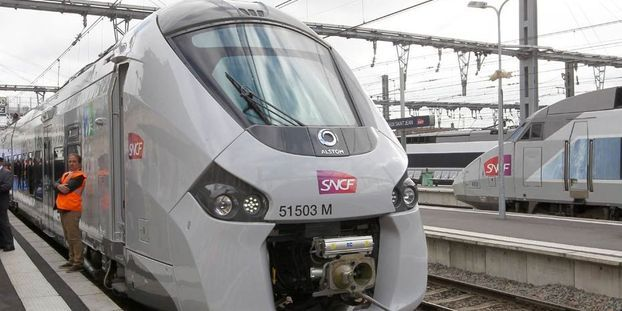
\includegraphics[width=\linewidth]{images/image9.jpeg}

Les ingénieurs de la SNCF de l\textquotesingle époque, qui ont définis le
cahier des charges et notamment les dimensions des nouvelles rames,
avaient omis de vérifier que celles-ci étaient conformes aux
infrastructures existantes. Aucune norme n\textquotesingle existant
alors quant à l\textquotesingle écartement entre le quai et la voie,
celui-ci pouvait légèrement varier d\textquotesingle une gare à
l\textquotesingle autre. Conséquence : 1300 quais (sur les 9000 que
comptent les gares françaises) ont eu besoin d'un rabotage de 1 à 2 cm !

\subsection{Cas n°3~: Voitures}\label{cas-n3-voitures}

Au début du XXème siècle, les véhicules peuvent être vus comme un
assemblage de pièces mécaniques. Il était donc assez simple de concevoir
et d\textquotesingle analyser ce type de système. Avec
l\textquotesingle arrivée de l\textquotesingle électronique, de
nouvelles fonctionnalités, cela va devenir plus complexe et nécessiter
de nouvelles méthodes.

Par exemple, si l\textquotesingle on compare la conception de la 2CV et
de la Dacia Lodgy, on peut voir l\textquotesingle augmentation du cahier
des charges, des fonctionnalités, de la cadence de production\ldots{}

\begin{longtable}[]{@{}
  >{\raggedright\arraybackslash}p{(\columnwidth - 4\tabcolsep) * \real{0.3292}}
  >{\raggedright\arraybackslash}p{(\columnwidth - 4\tabcolsep) * \real{0.3390}}
  >{\raggedright\arraybackslash}p{(\columnwidth - 4\tabcolsep) * \real{0.3319}}@{}}
\toprule\noalign{}
\begin{minipage}[b]{\linewidth}\raggedright
Le passé
\end{minipage} & \begin{minipage}[b]{\linewidth}\raggedright
Le présent
\end{minipage} & \begin{minipage}[b]{\linewidth}\raggedright
Le futur proche
\end{minipage} \\
\midrule\noalign{}
\endhead
\bottomrule\noalign{}
\endlastfoot
La 2CV & \textbf{La Dacia Lodgy} & \textbf{Le véhicule autonome} \\
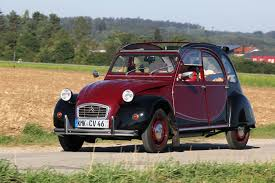
\includegraphics[width=\linewidth]{images/image10.jpeg}
&
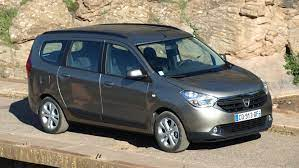
\includegraphics[width=\linewidth]{images/image11.jpeg}
&
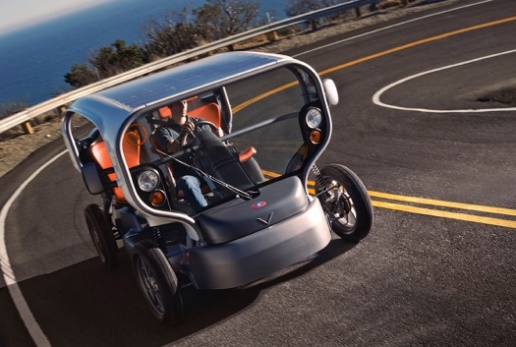
\includegraphics[width=\linewidth]{images/image12.jpeg} \\
7 à 11 années de conception & 3 ans & En cours de prototypage \\
167 419 vendues en 1964 (apogée) & 240 700 vendues en 2018 & \\
Pas d\textquotesingle électronique & Des dizaines de calculateurs &
Électronique embarquée \\
Dix lignes d\textquotesingle exigences textuelles & 1 million
d\textquotesingle exigences & \\
Aucune aide à la conduite & De nombreuses aides de série & Pas de
conducteur \\
Aucun standard à respecter & De nombreux standards et réglementations &
Réglementations en cours d'élaboration \\
\end{longtable}

De manière générale, le Standish Group a établi en 2015 que les
principales causes de succès ou d\textquotesingle échecs
d\textquotesingle un projet sont liées aux exigences (un besoin est une
exigence de besoin) :

\begin{longtable}[]{@{}
  >{\raggedright\arraybackslash}p{(\columnwidth - 4\tabcolsep) * \real{0.2888}}
  >{\raggedright\arraybackslash}p{(\columnwidth - 4\tabcolsep) * \real{0.4347}}
  >{\raggedright\arraybackslash}p{(\columnwidth - 4\tabcolsep) * \real{0.2766}}@{}}
\toprule\noalign{}
\begin{minipage}[b]{\linewidth}\raggedright
\textbf{Facteurs d\textquotesingle échecs}
\end{minipage} & \begin{minipage}[b]{\linewidth}\raggedright
\textbf{Causes racines}
\end{minipage} & \begin{minipage}[b]{\linewidth}\raggedright
\textbf{Facteurs de succès}
\end{minipage} \\
\midrule\noalign{}
\endhead
\bottomrule\noalign{}
\endlastfoot
37 \% & Besoins, exigences & 40 \% \\
9 \% & Projet, ressources & 23 \% \\
8 \% & Gestion des données techniques & 14 \% \\
11 \% & Technique, technologie & 9 \% \\
\end{longtable}

\begin{bob}[title=Le conseil de Bob]

Il faut bien définir le besoin et les exigences que doivent vérifier mon
produit~!
\end{bob}

\section{\texorpdfstring{Typologie des systèmes
}{Typologie des systèmes }}\label{typologie-des-systuxe8mes}

\subsection{Définition}\label{duxe9finition}

\textbf{Système}~: Un système est un ensemble d\textquotesingle éléments
en interaction, organisés pour atteindre un ou plusieurs résultats,
quantifiables en termes de performance.

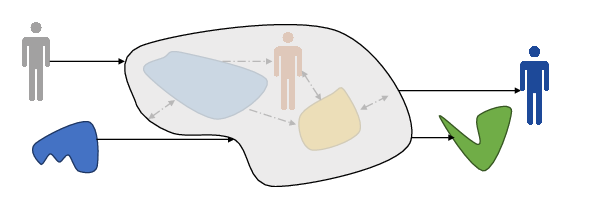
\includegraphics[width=\linewidth]{images/image14.png}

\emph{Source : ISO 15288.}

Il existe deux grandes catégories de systèmes :

\begin{itemize}
\item
  les systèmes naturels (système solaire) ;
\item
  les systèmes artificiels, créés par l\textquotesingle Homme pour
  remplir une fonction précise.
\end{itemize}

\subsection{Les systèmes en SII}\label{les-systuxe8mes-en-sii}

Au cours de cette année, nous nous focaliserons sur trois aspects du
système qui nécessiteront des vues et certains types de modèles :

\begin{itemize}
\item
  Le \textbf{système souhaité}, défini par un ensemble de documents dont
  le cahier des charges.
\item
  Le \textbf{système simulé}, défini numériquement par un ou des
  fichiers exécutables par un ou des logiciels de simulation.
\item
  Le \textbf{système réel}, dont une version peut être disponible
  physiquement ou virtuellement dans le laboratoire.
\end{itemize}

\paragraph*{Performances d'un système, l'ensemble du processus
industriel va faire naître des
:}\label{performances-dun-systuxe8me-lensemble-du-processus-industriel-va-faire-nauxeetre-des}
\addcontentsline{toc}{paragraph}{Performances d'un système, l'ensemble
du processus industriel va faire naître des :}

\begin{itemize}
\item
  écarts entre les performances du produit réalisé par l'industriel et
  les performances du produit désiré par le client ;
\item
  écarts entre les performances du produit conçu par le bureau d'étude
  et les performances du produit réalisé par l'atelier de fabrication ;
\item
  écarts entre les simulations issues du bureau d'étude et les
  performances réelles du système ; entre les performances du produit
  commercialisé et les attentes du client.
\end{itemize}

Le but des Sciences Industrielles de l'Ingénieur (et des industriels)
est de quantifier et maîtriser l'ensemble de ces écarts pour atteindre
la satisfaction du client la plus grande possible.

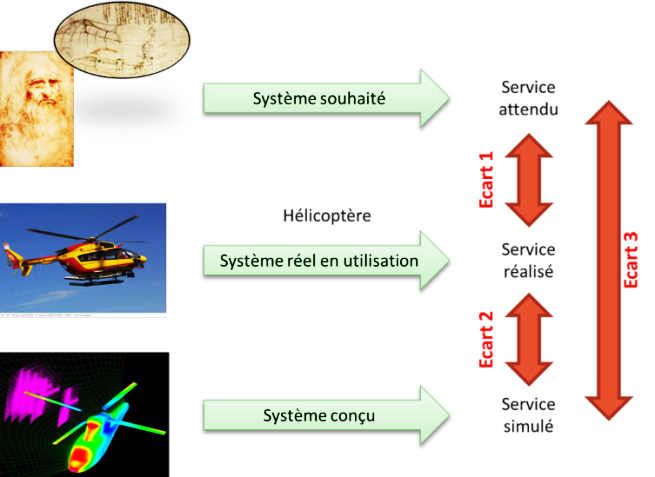
\includegraphics[width=\linewidth]{images/image15.png}

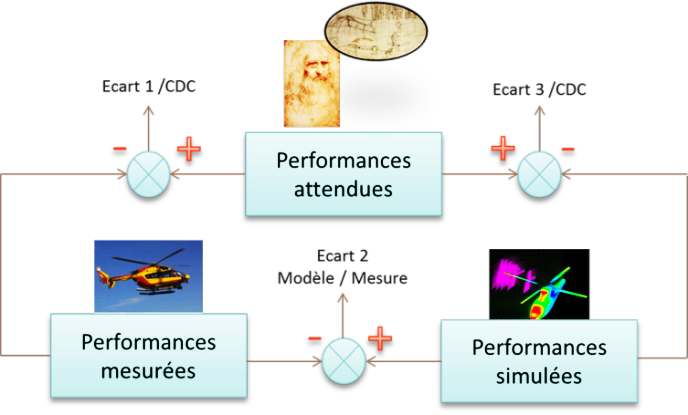
\includegraphics[width=\linewidth]{images/image16.png}

\emph{Modélisation des écarts}

\subsection{Cycle de vie}\label{cycle-de-vie}

Nous distinguerons ici deux visions du cycle de vie d'un système, très
supplémentaire et dont la finalité diffère selon l'usage~:

\begin{itemize}
\item
  le cycle de vie d'un produit, défini par la norme ISO 14040, et utile
  à des fins d'analyse du cycle de vie et de limitation des impacts
  environnementaux tout au long du cycle de vie~;
\item
  le cycle de vie d'un système, défini par la norme ISO 15288, et utile
  à mettre en œuvre l'IS dans une démarche de conception.
\end{itemize}

Le cycle de vie commence à l'extraction des matières premières jusqu'à
son élimination (fin de vie ou recyclage). La prise en compte de chacune
de ces étapes pour l'analyse des différents impacts est primordiale,
afin d'éviter un déplacement des problèmes (transfert d'impact).

La démarche d'éco-conception ou d'éco-construction s'inscrit totalement
dans ce cycle.

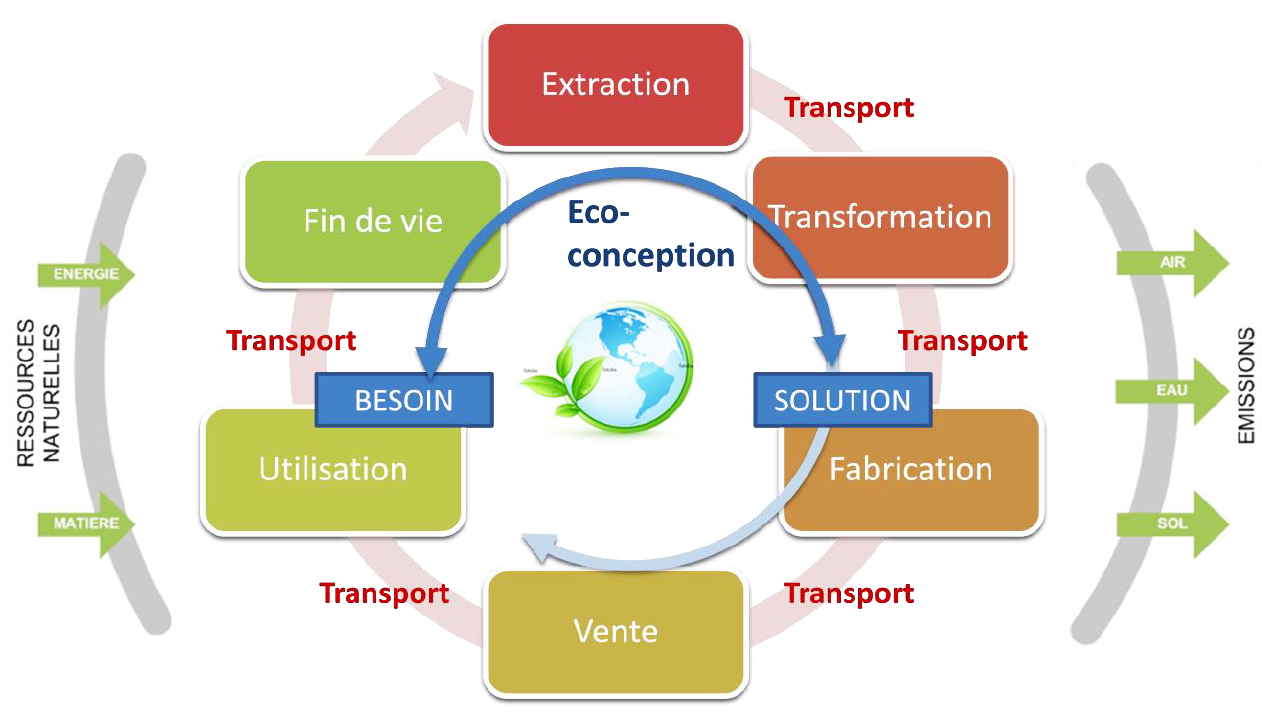
\includegraphics[width=\linewidth]{images/image17.png}

A chaque étape :

\begin{itemize}
\item
  un produit consomme de l'énergie et des matières premières non
  renouvelables ;
\item
  un produit crée des impacts sur l'air, l'eau, le sol.
\end{itemize}

\paragraph*{Les impacts
environnementaux}\label{les-impacts-environnementaux}
\addcontentsline{toc}{paragraph}{Les impacts environnementaux}

Les impacts environnementaux sont classés en 3 familles d'impact : les
ressources naturelles non renouvelables, les pollutions et les
nuisances. A chaque impact correspond alors une unité de référence.

\begin{longtable}[]{@{}
  >{\raggedright\arraybackslash}p{(\columnwidth - 4\tabcolsep) * \real{0.1802}}
  >{\raggedright\arraybackslash}p{(\columnwidth - 4\tabcolsep) * \real{0.5421}}
  >{\raggedright\arraybackslash}p{(\columnwidth - 4\tabcolsep) * \real{0.2777}}@{}}
\toprule\noalign{}
\begin{minipage}[b]{\linewidth}\raggedright
\textbf{Familles d'impacts}
\end{minipage} & \begin{minipage}[b]{\linewidth}\raggedright
\textbf{Impacts}
\end{minipage} & \begin{minipage}[b]{\linewidth}\raggedright
\textbf{Substance ou unité de référence}
\end{minipage} \\
\midrule\noalign{}
\endhead
\bottomrule\noalign{}
\endlastfoot
\multirow{2}{=}{Ressources naturelles

non renouvelables} & Consommation d'énergie non renouvelable & MégaJoule
(\emph{MJ}) \\
& Consommation de ressources naturelles non renouvelables & Antimoine
(\emph{Sb}) \\
\multirow{5}{=}{Pollutions} & Gaz à Effet de Serre (GES) ou Global

Warming Potential (GWP) & Dioxyde de carbone
(\emph{CO\textsubscript{2}}) \\
& Acidification liée aux pluies acides & Dioxyde de soufre
(\emph{SO\textsubscript{2}}) \\
& Eutrophisation liée à l'enrichissement des milieux aquatiques en sels
nutritifs & Composé phosphaté (\emph{PO} 3-4) \\
& Dégradation de la couche d'ozone & Fréon 11 (CFC-11) \\
& Toxicité d'une substance sur les organismes (écotoxicité) & 1,4
Dichlorobenzène (1,4 DCB) \\
\multirow{3}{=}{Nuisances} & Acoustiques & Decibel (dB) \\
& Visuelles & \\
& Olfactives & \\
\end{longtable}

Pour comparer les différents impacts environnementaux, on utilise
généralement le taux de CO\textbf{\textsubscript{2}} équivalent émis.

'\,'

\begin{longtable}[]{@{}
  >{\raggedright\arraybackslash}p{(\columnwidth - 2\tabcolsep) * \real{0.5247}}
  >{\raggedright\arraybackslash}p{(\columnwidth - 2\tabcolsep) * \real{0.4753}}@{}}
\toprule\noalign{}
\begin{minipage}[b]{\linewidth}\raggedright
Matériau
\end{minipage} & \begin{minipage}[b]{\linewidth}\raggedright
Émissions équivalentes de CO\textsubscript{2} en kg par tonne produite
\end{minipage} \\
\midrule\noalign{}
\endhead
\bottomrule\noalign{}
\endlastfoot
Verre bouteille & 120 \\
Ciment & 250 \\
Acier & 300 à 850 selon le \% de ferrailles \\
Papier-carton & 300 à 500 \\
Plastiques (polyéthylène, polystyrène, \ldots) & 500 à 1600 \\
Aluminium & 600 à 3000 selon le \% de déchets \\
\end{longtable}


\section{L'approche Ingénierie
Système}\label{lapproche-inguxe9nierie-systuxe8me}

\subsection{Définition}\label{duxe9finition-1}

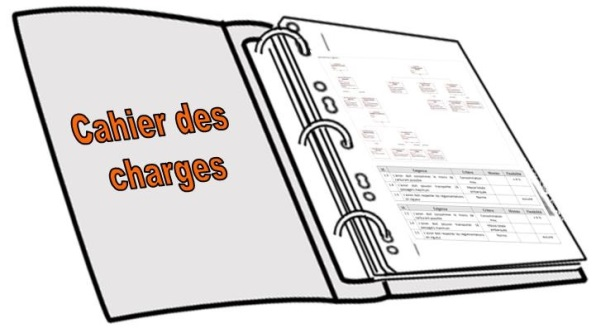
\includegraphics[width=\linewidth]{images/image20.jpeg}

\textbf{Ingénierie système} : ~Démarche méthodologique coopérative et
interdisciplinaire qui englobe l'ensemble des activités adéquates pour
concevoir, développer, faire évoluer et vérifier un ensemble de
produits, processus et compétences humaines apportant une solution
économique et performante aux besoins des parties prenantes et
acceptable par tous (inspiré de IEEE 1220).~

\textbf{Définition}

L'ensemble des exigences qui doivent être satisfaites par le système et
leurs caractéristiques (critère et niveau) sont regroupées dans le
\textbf{cahier des charges.}

\paragraph*{Pourquoi l'Ingénierie
Système}\label{pourquoi-linguxe9nierie-systuxe8me}
\addcontentsline{toc}{paragraph}{Pourquoi l'Ingénierie Système}

Les moyens de plus en plus performants pour piloter (coût, délai,
qualité, impact environnemental, etc.) les différentes phases de
conception, d'intégration et de validation de systèmes apportant une
solution économique et performante aux besoins d'un client.

Cet objectif est atteint grâce à l'Ingénierie Système :

\begin{enumerate}
\def\labelenumi{\alph{enumi}.}
\setcounter{enumi}{14}
\item
  une prise en compte précise de la demande du client,
\end{enumerate}

\begin{enumerate}
\def\labelenumi{\alph{enumi}.}
\setcounter{enumi}{14}
\item
  une coordination efficiente des nombreux métiers sollicités lors du
  développement,
\end{enumerate}

\begin{enumerate}
\def\labelenumi{\alph{enumi}.}
\setcounter{enumi}{14}
\item
  une décomposition ordonnée de l'architecture du système,
\end{enumerate}

\begin{quote}
o la prise en compte, tout au long du projet, de son cycle de vie.
\end{quote}

\subsection{Produit et besoin}\label{produit-et-besoin}

Pour se développer et survivre, l'entreprise doit vendre les systèmes
qu'elle produit. Le \emph{\textbf{client achète un système si celui-ci
répond à un besoin et le satisfait}}, il y a donc obligation pour
l'entreprise d'ajuster le système en fonction du besoin du client.

Le client achète le produit si celui-ci répond à un \textbf{besoin} et
le satisfait, il y a donc obligation pour l'entreprise d'ajuster le
produit en fonction du besoin du client. C'est donc pour elle un enjeu
vital de :

\begin{itemize}
\item
  \textbf{percevoir et formaliser} \textbf{le besoin du client.}
\item
  \textbf{caractériser le taux de satisfaction attendu.}
\end{itemize}

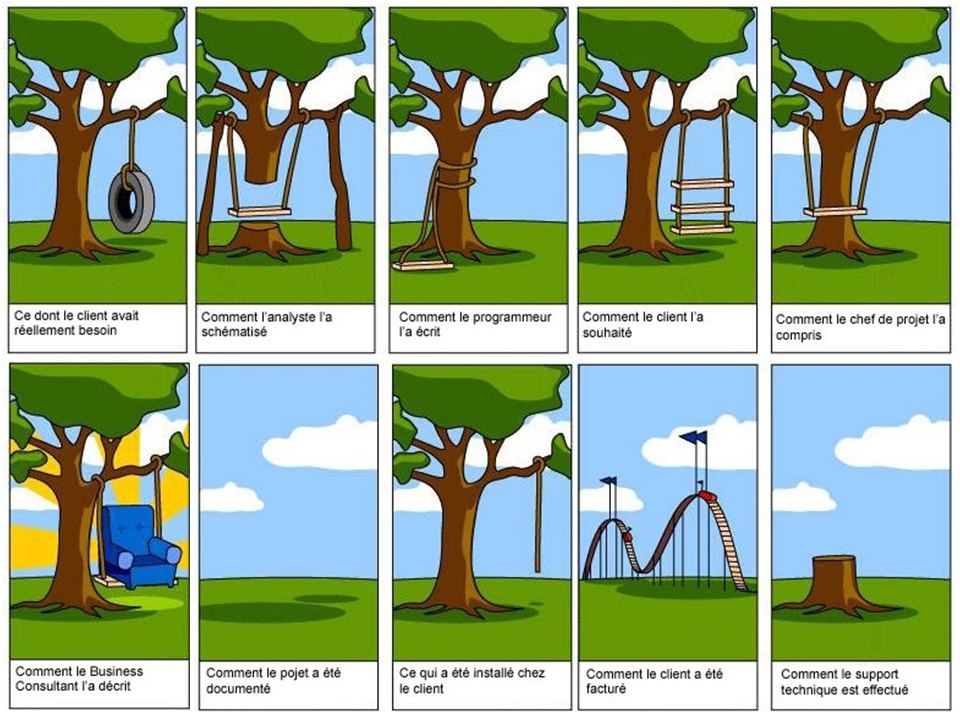
\includegraphics[width=\linewidth]{images/image26.png}Il
est très important que les différentes parties prenantes aient la même
vision du système qui va être conçu. L\textquotesingle enjeu est
d\textquotesingle éviter que le système conçu soit différent de celui
souhaité...

J'aimerais une balançoire

Et si elle était durable~?

\emph{Intérêt de l'analyse du besoin -- Source~: IBM}

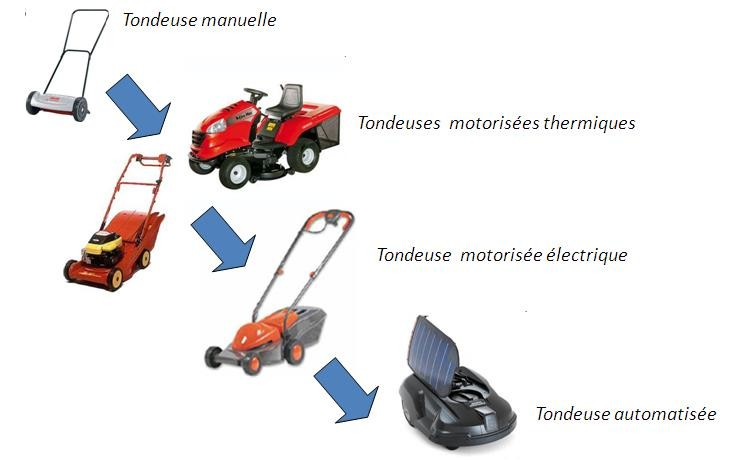
\includegraphics[width=\linewidth]{images/image30.jpeg}L'entreprise
peut pour cela utiliser des enquêtes, sondages ou études de marché, mais
ces outils ne suffisent pas pour analyser correctement le besoin.

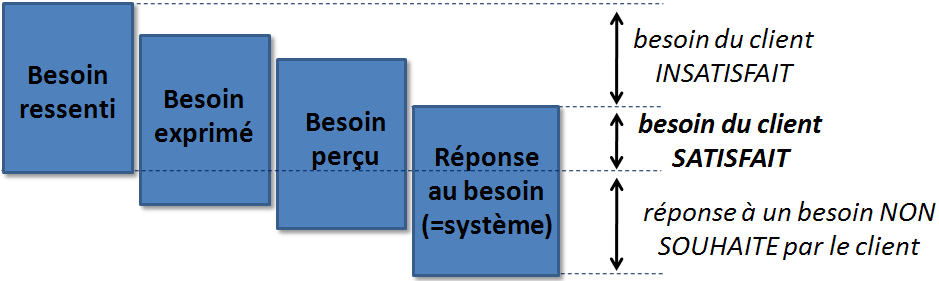
\includegraphics[width=\linewidth]{images/image32.png}Cela
est d'autant plus difficile que le client est sensible à
l'\emph{\textbf{évolution du contexte économique, social et
environnemental}} ainsi qu'au \emph{\textbf{degré d'innovation}}, le
besoin évolue donc constamment (besoin d'un nouveau portable, \ldots).

L'entreprise doit anticiper sur les besoins de demain pour rester
compétitive\textbf{,} il faut donc que \emph{\textbf{la réponse au
besoin évolue aussi.}}

\subsection{Processus global}\label{processus-global}

L'ingénierie système consiste donc en une pratique permettant de
concevoir intelligemment un système complexe. Voici comment ces
différentes activités peuvent s'enchainer.

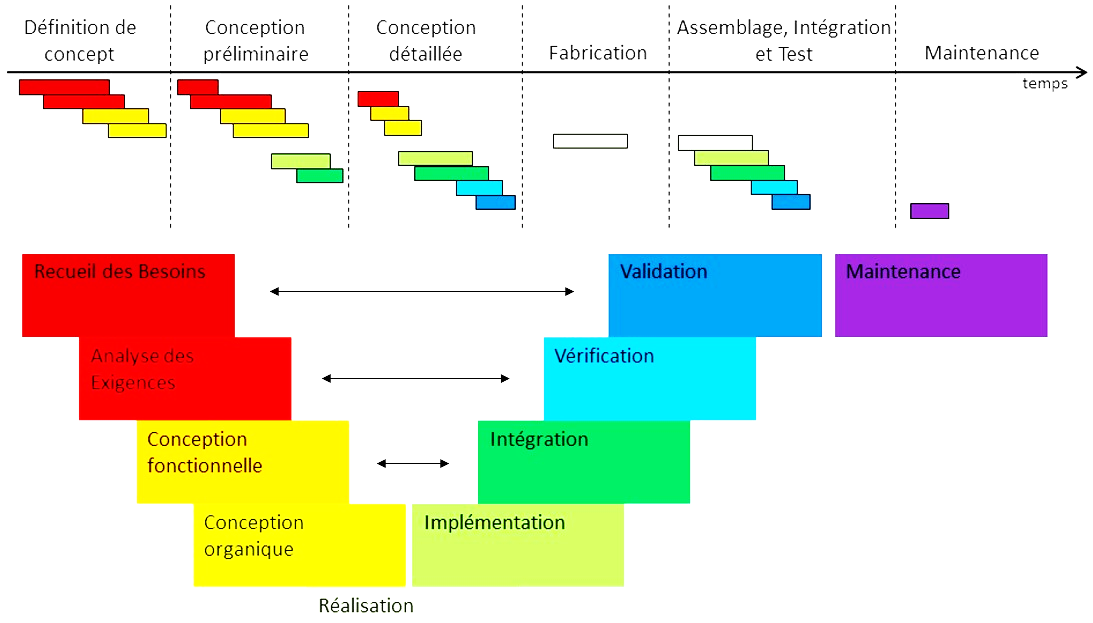
\includegraphics[width=\linewidth]{images/image33.png}

Processus de Conception. Sources : NASA et ISO 15288

\section{Le langage et les diagrammes
SysML}\label{le-langage-et-les-diagrammes-sysml}


\includegraphics[width=0.25\linewidth]{images/image34.png}Le
langage SysML (System Modeling Language) permet dans les différentes
phases de vie d'un produit (conception, intégration, validation,
évolution, \ldots) de faciliter~:

\begin{itemize}
\item
  la collaboration transdisciplinaire,
\item
  l'interprétation, le stockage et le partage des données,
\item
  les modélisations communes,
\end{itemize}

SysML s'articule autour de neuf diagrammes, chacun d'eux étant dédié à
la représentation de concepts particuliers. Ces types de diagrammes sont
répartis par l'OMG (Object Management Group) en trois grands groupes :

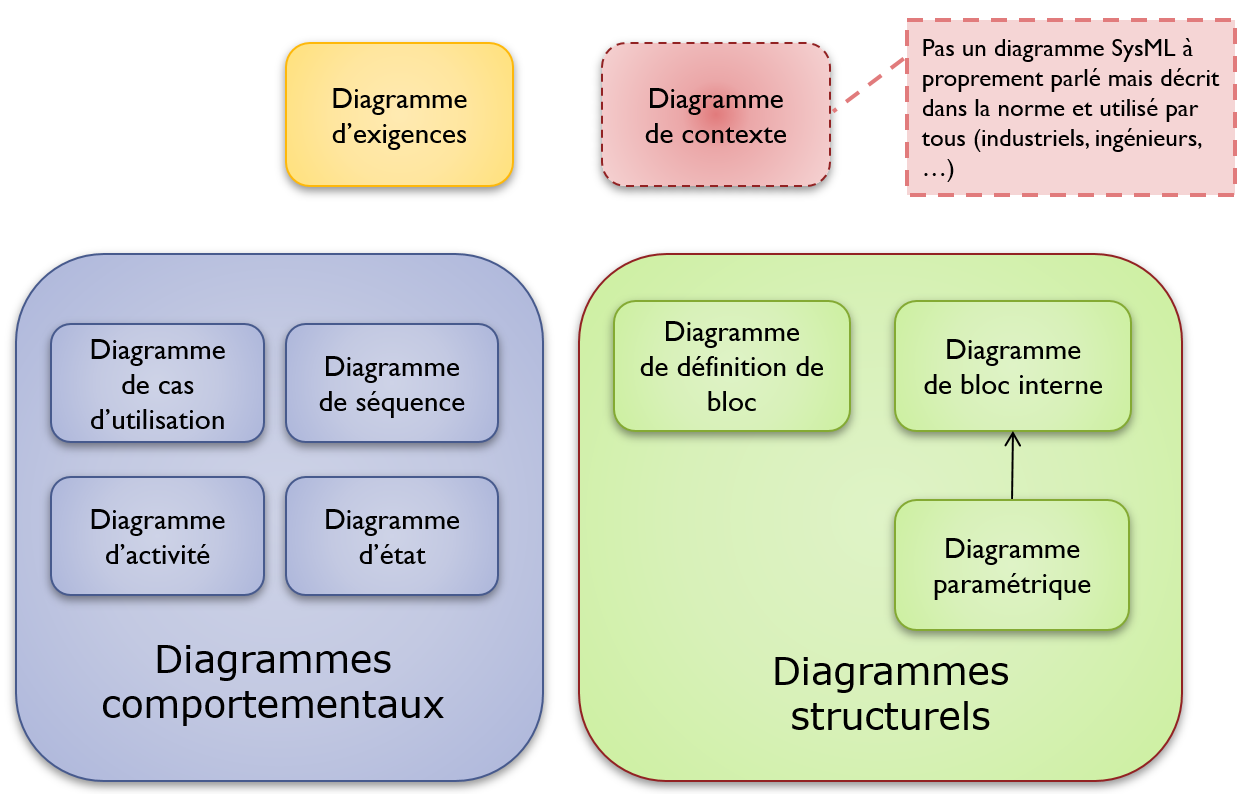
\includegraphics[width=\linewidth]{images/image35.png}

\emph{Les différents diagrammes SysML regroupés par catégories}

\begin{itemize}
\item
  Le \textbf{diagramme des exigences}~: diagramme transversal, puisque
  chaque élément modélisé est en lien avec au moins une exigence, qui
  montre les besoins/exigences du système et leurs relations
\item
  Les diagrammes comportementaux :
\end{itemize}

\begin{itemize}
\item
  \textbf{diagramme de cas d'utilisation}~: montre les services rendus
  par le système, en interaction avec les acteurs concernés~;
\item
  \textbf{diagramme de séquence}~: montre le déroulement temporel des
  interactions entre le système et son environnement (boîte noire),
  voire au sein du système lui-même (boîte blanche)~;
\item
  \textbf{diagramme d'état}~: montre les différents états du système et
  leurs modes de changement~;
\item
  \textbf{diagramme d'activité}~: montre l'enchainement séquentiel des
  activités réalisées dans les états.
\end{itemize}


\boxreflexion{
\begin{enumerate}
  \item Définir le besoin d’un micro-onde.
  \item Définir le besoin du drone.
\end{enumerate}
}


\begin{itemize}
\item
  Les diagrammes structurels :
\end{itemize}

\begin{itemize}
\item
  \textbf{diagramme de définition de blocs}~: montre la structure du
  système sous forme de décomposition en éléments plus simples
  (sous-systèmes, blocs)~;
\item
  \textbf{diagramme de bloc interne}~: montre l'organisation interne des
  constituants et leurs interactions en termes d'échanges de flux MEI
  (Matière -- Energie -- Information)~;
\item
  diagramme paramétrique~: représente les contraintes des constituants,
  les équations qui les régissent ;
\item
  diagramme de packages~: montre l'organisation logique du modèle et les
  relations entre packages.
\end{itemize}

A ces trois grands groupes il convient d'y adjoindre le
\textbf{diagramme de contexte}, non référencé en tant que tel dans la
norme (il peut être fait avec un diagramme de définition de blocs ou de
bloc interne), mais évoqué dans celle-ci et largement utilisé en
pratique.

Une pratique largement répandue est d'utiliser des acronymes en lieu et
place des noms des diagrammes. Les acronymes et symboles employés dans
la suite de ce cours~sont les suivants :

\begin{longtable}[]{@{}
  >{\raggedright\arraybackslash}p{(\columnwidth - 8\tabcolsep) * \real{0.2564}}
  >{\raggedright\arraybackslash}p{(\columnwidth - 8\tabcolsep) * \real{0.2208}}
  >{\raggedright\arraybackslash}p{(\columnwidth - 8\tabcolsep) * \real{0.2101}}
  >{\raggedright\arraybackslash}p{(\columnwidth - 8\tabcolsep) * \real{0.1575}}
  >{\raggedright\arraybackslash}p{(\columnwidth - 8\tabcolsep) * \real{0.1551}}@{}}
\toprule\noalign{}
\begin{minipage}[b]{\linewidth}\raggedright
\textbf{Nom français}
\end{minipage} & \begin{minipage}[b]{\linewidth}\raggedright
\textbf{English name}
\end{minipage} & \begin{minipage}[b]{\linewidth}\raggedright
\textbf{Acronyme}
\end{minipage} & \begin{minipage}[b]{\linewidth}\raggedright
Autre acronyme
\end{minipage} & \begin{minipage}[b]{\linewidth}\raggedright
Symbole
\end{minipage} \\
\midrule\noalign{}
\endhead
\bottomrule\noalign{}
\endlastfoot
Diagramme d'exigences & \textbf{R}equirement \textbf{D}iagram &
\textbf{RD} & Req &

\includegraphics[width=\linewidth]{images/image36.png} \\
Diagramme de cas d'utilisation & \textbf{U}se \textbf{C}ase
\textbf{D}iagram & \textbf{UCD} & Uc &

\includegraphics[width=\linewidth]{images/image37.png} \\
Diagramme de séquence & \textbf{S}equence \textbf{D}iagram & \textbf{SD}
& Seq &
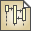
\includegraphics[width=\linewidth]{images/image38.png} \\
Diagramme d'états/transitions & \textbf{S}tate \textbf{M}achine
\textbf{D}iagram & \textbf{SMD} & Stm &

\includegraphics[width=\linewidth]{images/image39.png} \\
Diagramme d'activités & \textbf{A}ctivity \textbf{D}iagram & \textbf{AD}
& Act &

\includegraphics[width=\linewidth]{images/image40.png} \\
Diagramme de définition de blocs & \textbf{B}lock \textbf{D}efinition
\textbf{D}iagram & \textbf{BDD} & - &

\includegraphics[width=\linewidth]{images/image41.png} \\
Diagramme de blocs internes & \textbf{I}nternal \textbf{B}lock
\textbf{D}iagram & \textbf{IBD} & - &
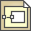
\includegraphics[width=\linewidth]{images/image42.png} \\
\end{longtable}

\subsection{Les objets et les
relations}\label{les-objets-et-les-relations}

SysML est un langage orienté objet, possédant chacun des attributs
spécifiques. La plupart des objets sont représentés par un rectangle
contenant~:

\begin{itemize}
\item
  une entête~: elle contient le stéréotype précisant la nature de
  l'objet (entre «~») ainsi que son nom~;
\item
  un (ou plusieurs) compartiment(s)~: précisant certaines propriétés
  spécifiques (un numéro d'identifiant et un texte pour une exigence~;
  les éléments (parts), les valeurs, les propriétés, les méthodes
  (opérations) pour un bloc, ...
\end{itemize}

Certains objets particuliers sont représentés par un symbole~: c'est le
cas des acteurs comme l'utilisateur (représenté par un bonhomme bâton,
ou «~sticky boy~»).

\begin{longtable}[]{@{}
  >{\raggedright\arraybackslash}p{(\columnwidth - 4\tabcolsep) * \real{0.3422}}
  >{\raggedright\arraybackslash}p{(\columnwidth - 4\tabcolsep) * \real{0.3310}}
  >{\raggedright\arraybackslash}p{(\columnwidth - 4\tabcolsep) * \real{0.3269}}@{}}
\toprule\noalign{}
\multicolumn{3}{@{}>{\raggedright\arraybackslash}p{(\columnwidth - 4\tabcolsep) * \real{1.0000} + 4\tabcolsep}@{}}{%
\begin{minipage}[b]{\linewidth}\raggedright
\textbf{Exemples d'objets en langage SysML}
\end{minipage}} \\
\midrule\noalign{}
\endhead
\bottomrule\noalign{}
\endlastfoot
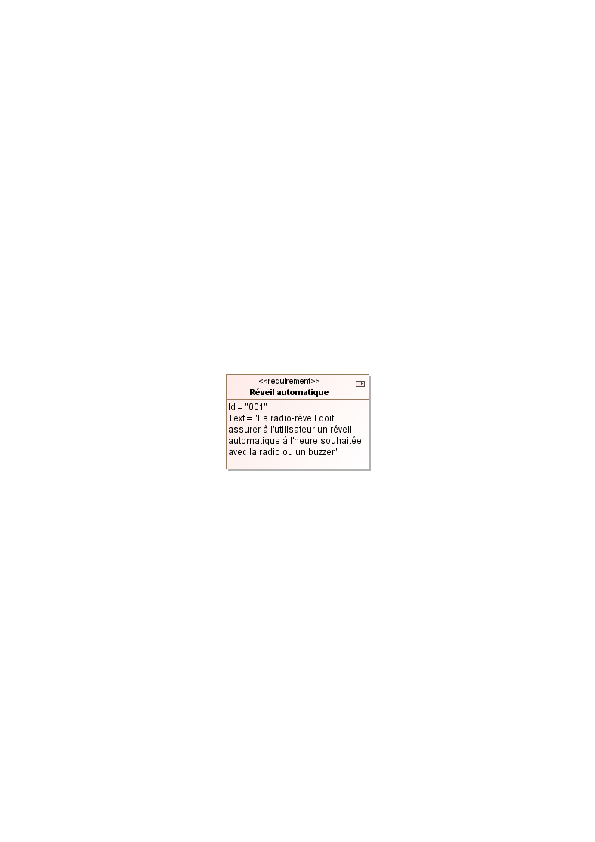
\includegraphics[width=\linewidth]{images/image43.png}
&
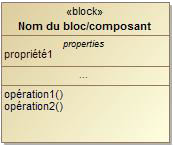
\includegraphics[width=\linewidth]{images/image44.png}
& 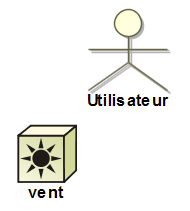
\includegraphics{images/image45.png} \\
Une exigence & Un bloc & Des acteurs \\
\end{longtable}

Ces objets peuvent être en relation les uns les autres, par le biais
d'un lien exprimant le type de relation entre les deux objets. Très
souvent, il est basé sur une flèche (indiquant le sens de lecture de la
relation), les relations se différenciant les unes des autres par~:

\begin{itemize}
\item
  le type de trait~: plein ou en pointillé~;
\item
  le type de flèche~: sans, avec flèche pleine ou ouverte~;
\item
  le symbole attaché à l'objet «~parent~», l'objet relié étant considéré
  comme l'~«~enfant~»~;
\item
  un stéréotype éventuel~: pour les liens en pointillé, précisant la
  nature de celui-ci.
\end{itemize}

\begin{longtable}[]{@{}
  >{\raggedright\arraybackslash}p{(\columnwidth - 6\tabcolsep) * \real{0.3166}}
  >{\raggedright\arraybackslash}p{(\columnwidth - 6\tabcolsep) * \real{0.1855}}
  >{\raggedright\arraybackslash}p{(\columnwidth - 6\tabcolsep) * \real{0.2707}}
  >{\raggedright\arraybackslash}p{(\columnwidth - 6\tabcolsep) * \real{0.2271}}@{}}
\toprule\noalign{}
\multicolumn{4}{@{}>{\raggedright\arraybackslash}p{(\columnwidth - 6\tabcolsep) * \real{1.0000} + 6\tabcolsep}@{}}{%
\begin{minipage}[b]{\linewidth}\raggedright
\textbf{Principaux liens entre objets en langage SysML}\footnote{Non
  valables pour les liens entre états et les liens entre activités, qui
  ont leur syntaxe et leur sémantique propre.}
\end{minipage}} \\
\midrule\noalign{}
\endhead
\bottomrule\noalign{}
\endlastfoot
Symbole & Nom & Description & Remarque \\
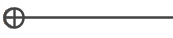
\includegraphics{images/image46.png} &
Contenance & L'objet de gauche contient l'objet de droite. & Concerne
uniquement les exigences \\
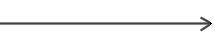
\includegraphics{images/image47.png} &
Association & Les deux objets sont associés entre eux & La nature de
l'association peut être précisée sur le lien \\
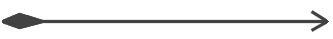
\includegraphics{images/image48.png} &
Composition & L'objet de gauche est composé de l'objet de droite. &
Concerne principalement les blocs \\
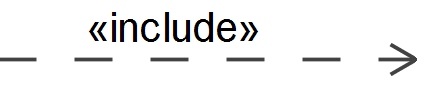
\includegraphics{images/image49.png} &
Inclusion & L'objet de gauche inclut l'objet de droite. & Concerne
uniquement les cas d'utilisations \\
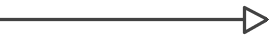
\includegraphics{images/image50.png} &
Spécialisation/

Généralisation & L'objet de gauche est une spécialisation de l'objet de
droite & Concerne tous les types d'objets \\
\end{longtable}

\subsubsection[Exemple avec un
drone]{\texorpdfstring{\protect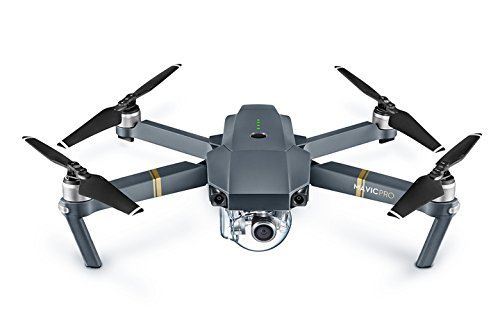
\includegraphics[width=\linewidth]{images/image51.jpeg}Exemple
avec un
drone}{DJI - Mavic Pro Drone \textbar{} Drone Quadricoptère Portable \& Pliable avec Caméra \textbar{} Offre 27-Min de Vol \textbar{} Gimbal 3-Axis \& Caméra 4K \textbar{} Design Élégant \textbar{} Photos \& Vidéos enExemple avec un drone}}\label{dji---mavic-pro-drone-drone-quadricoptuxe8re-portable-pliable-avec-camuxe9ra-offre-27-min-de-vol-gimbal-3-axis-camuxe9ra-4k-design-uxe9luxe9gant-photos-viduxe9os-enexemple-avec-un-drone}

Dans la suite de ce cours, nous prendrons l'exemple suivi d'un drone de
loisir type Mavic de Dji ou drone Parrot.

\paragraph*{Éliciter et analyser les besoins de parties prenantes -- Use
Case}\label{uxe9liciter-et-analyser-les-besoins-de-parties-prenantes-use-case}
\addcontentsline{toc}{paragraph}{Éliciter et analyser les besoins de
parties prenantes -- Use Case}

Il est donc maintenant possible d\textquotesingle éliciter (ie :
comprendre et de modéliser) les besoins des parties prenantes et de les
analyser. Pour cela, il faut déterminer les services attendus en se
basant sur les différents acteurs pour chaque phase du cycle de vie.
Cela va ainsi permettre que les différentes parties prenantes soient
d\textquotesingle accord sur le système à concevoir. Cela se fait à
l\textquotesingle aide d\textquotesingle un diagramme SysML nommé
\textbf{UseCase} Diagram (Diagramme des Cas
d\textquotesingle utilisation). Il est possible d\textquotesingle en
dresser un global ou de les raffiner en en réalisant un pour chaque
phase du cycle de vie du système.

Les cas d\textquotesingle utilisation doivent être écrits comme un verbe
+ complément. De plus, les acteurs principaux sont placés à gauche afin
de faciliter la compréhension.

Pour trouver les cas d'utilisations, il est possible de dire~:
«~l'utilisateur veut que le système permette de\ldots.~».

'\,'

\begin{longtable}[]{@{}
  >{\raggedright\arraybackslash}p{(\columnwidth - 2\tabcolsep) * \real{0.1227}}
  >{\raggedright\arraybackslash}p{(\columnwidth - 2\tabcolsep) * \real{0.8773}}@{}}
\toprule\noalign{}
\begin{minipage}[b]{\linewidth}\raggedright
\begin{quote}

\includegraphics[width=\linewidth]{images/image52.png}
\end{quote}
\end{minipage} & \begin{minipage}[b]{\linewidth}\raggedright
\begin{enumerate}
\def\labelenumi{\arabic{enumi}.}
\item
  Définir le besoin d'un micro-onde.
\item
  Définir le besoin du drone
\end{enumerate}
\end{minipage} \\
\midrule\noalign{}
\endhead
\bottomrule\noalign{}
\endlastfoot
\end{longtable}

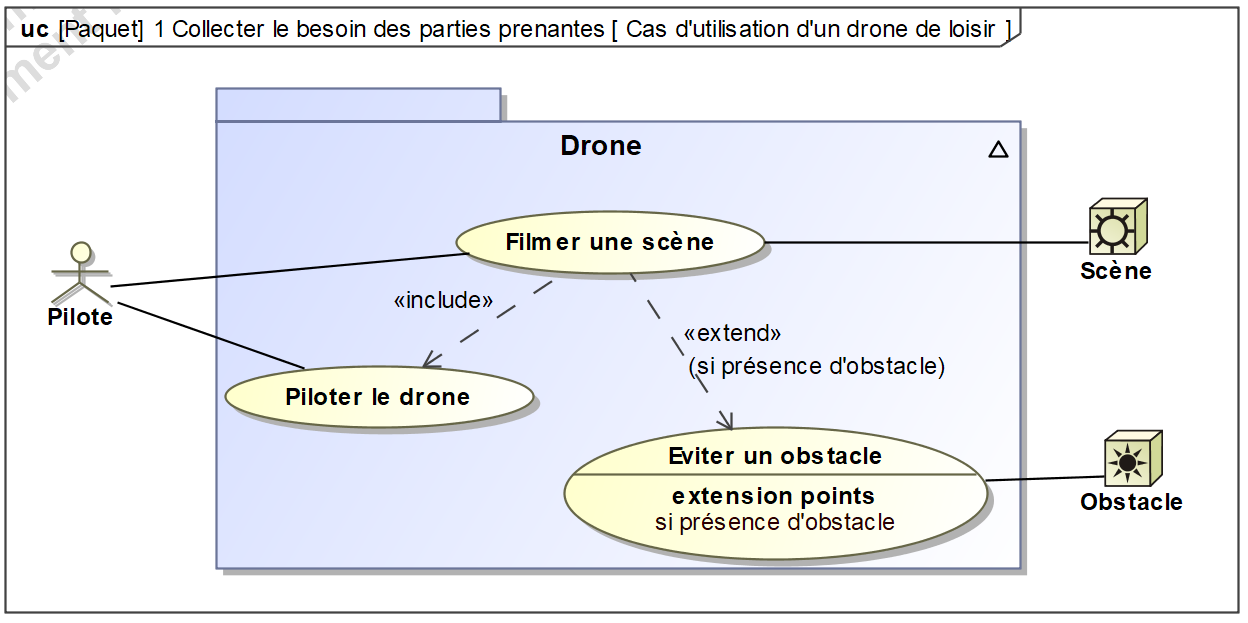
\includegraphics[width=\linewidth]{images/image3.png}

\paragraph*{Définir l\textquotesingle objectif du système et ses
frontières -- BDD
contexte}\label{duxe9finir-lobjectif-du-systuxe8me-et-ses-frontiuxe8res-bdd-contexte}
\addcontentsline{toc}{paragraph}{Définir l\textquotesingle objectif du
système et ses frontières -- BDD contexte}

Afin de fournir un cahier des charges fonctionnel sur lequel tout le
monde est d\textquotesingle accord, il faut définir le contexte
opérationnel du système.

Tout d\textquotesingle abord, la mission du système doit être définie.
Cela peut se résumer en une phrase définissant l'intérêt global du
système

Ensuite, il est possible de dresser le cycle de vie attendu du système
en n\textquotesingle oubliant pas les phases de maintenance et de
retrait à l\textquotesingle aide d\textquotesingle un diagramme
d\textquotesingle état comme cela a été mentionné précédemment.

Enfin, pour chaque phase du cycle de vie, il est possible de déterminer
tous les interacteurs dans un diagramme de contexte. Cela se fait par un
diagramme de blocs en SysML. Celui-ci présente les différents éléments
composant le sursystème du système (contexte d'utilisation) pour une
phase de vie.

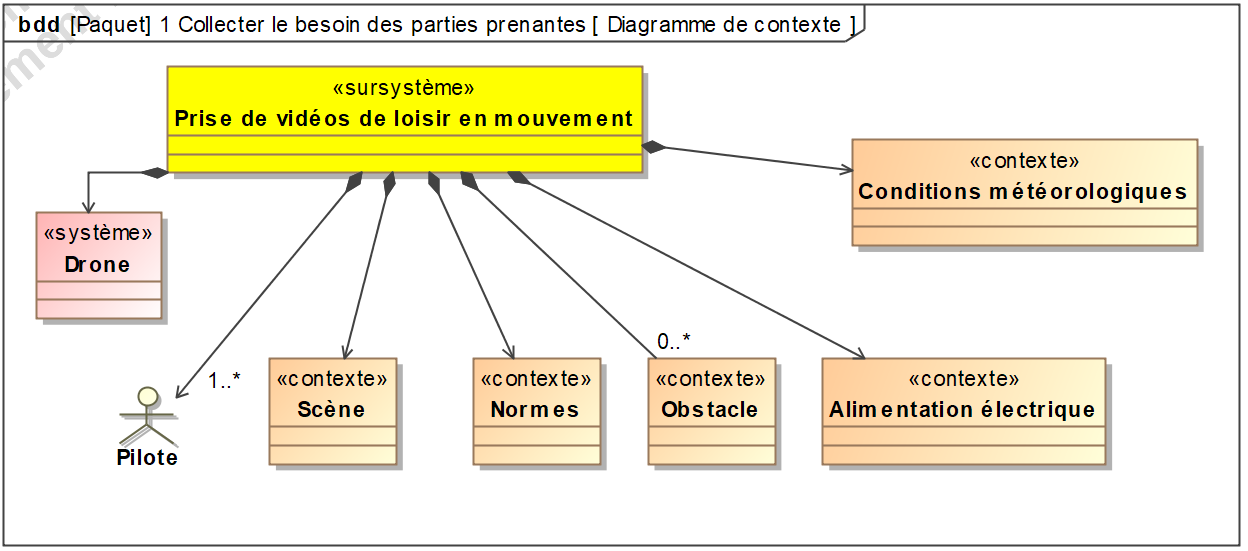
\includegraphics[width=\linewidth]{images/image53.png}

\paragraph*{Diagramme de contexte d\textquotesingle un drone de
loisir}\label{diagramme-de-contexte-dun-drone-de-loisir}
\addcontentsline{toc}{paragraph}{Diagramme de contexte
d\textquotesingle un drone de loisir}

Ainsi, pour le drone de loisir dans le contexte de prise de vidéos de
loisir en mouvement, plusieurs interacteurs sont présents~: au moins un
pilote, une scène, des normes, possiblement un ou plusieurs obstacles,
une alimentation électrique et des conditions météorologiques.

Ensuite, pour chaque cas d\textquotesingle utilisation, il est possible
de déterminer un diagramme de séquence permettant de déterminer les
interactions entre le système et les interacteurs.

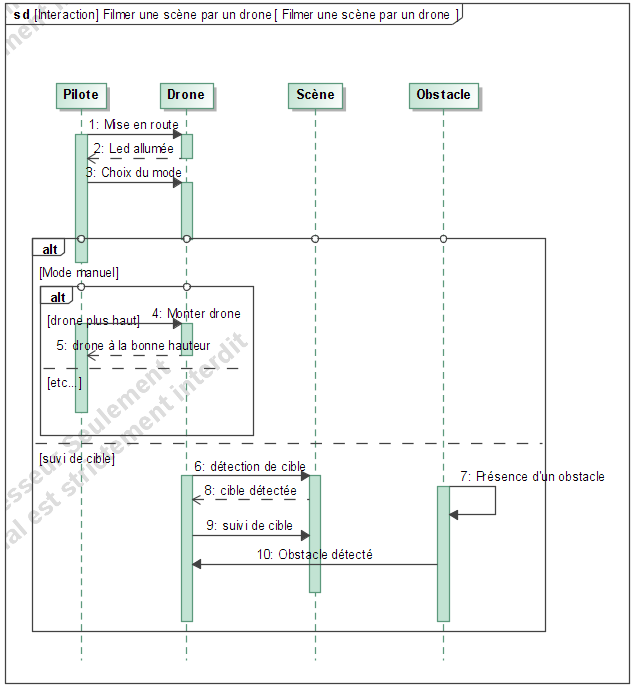
\includegraphics[width=\linewidth]{images/image54.png}

\emph{Exemple d\textquotesingle un diagramme de séquence concernant
l\textquotesingle action de filmer par un drone}

Cela ressemble à un storyboard de cinéma avec toutes les actions à
mener.

\paragraph*{Élaborer les exigences des parties prenantes -
Req}\label{uxe9laborer-les-exigences-des-parties-prenantes---req}
\addcontentsline{toc}{paragraph}{Élaborer les exigences des parties
prenantes - Req}

Maintenant que le contexte opérationnel et les services attendus ont été
définis, il est possible de rédiger l\textquotesingle ensemble des
exigences des parties prenantes dans le cahier des charges fonctionnel.
\textbf{Une règle de nommage est d\textquotesingle exprimer les
exigences par une phrase avec le verbe devoir ou une phrase à
l\textquotesingle infinitif.}

Une bonne exigence est MUST soit Mesurable, Utile, Simple, Traçable (ou
Testable).

'\,'

Pour synthétiser ce travail, on peut utiliser un diagramme des exigences
(req) en SysML :

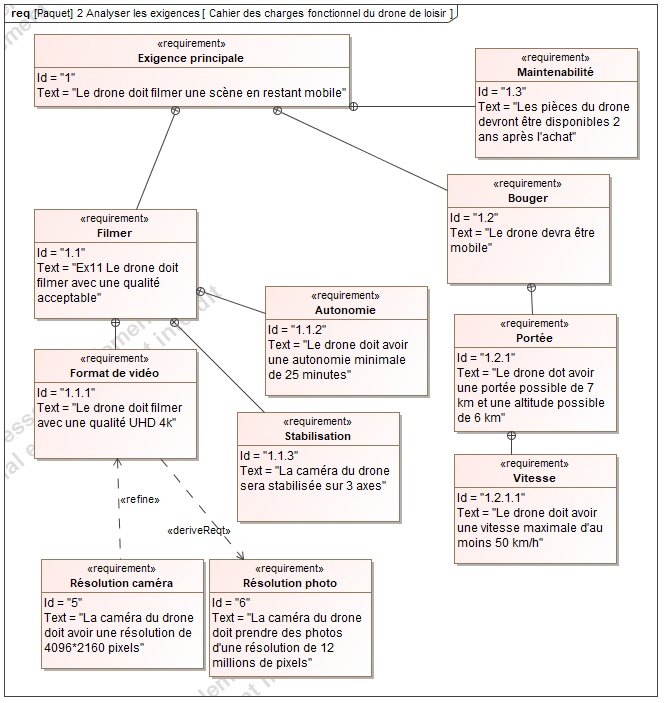
\includegraphics[width=\linewidth]{images/image55.png}

\paragraph*{Définir la décomposition fonctionnelle -- BDD
système}\label{duxe9finir-la-duxe9composition-fonctionnelle-bdd-systuxe8me}
\addcontentsline{toc}{paragraph}{Définir la décomposition fonctionnelle
-- BDD système}

A l'aide du cahier des charges et du patron de conception, il est
possible de déterminer une décomposition fonctionnelle du système
souhaité.

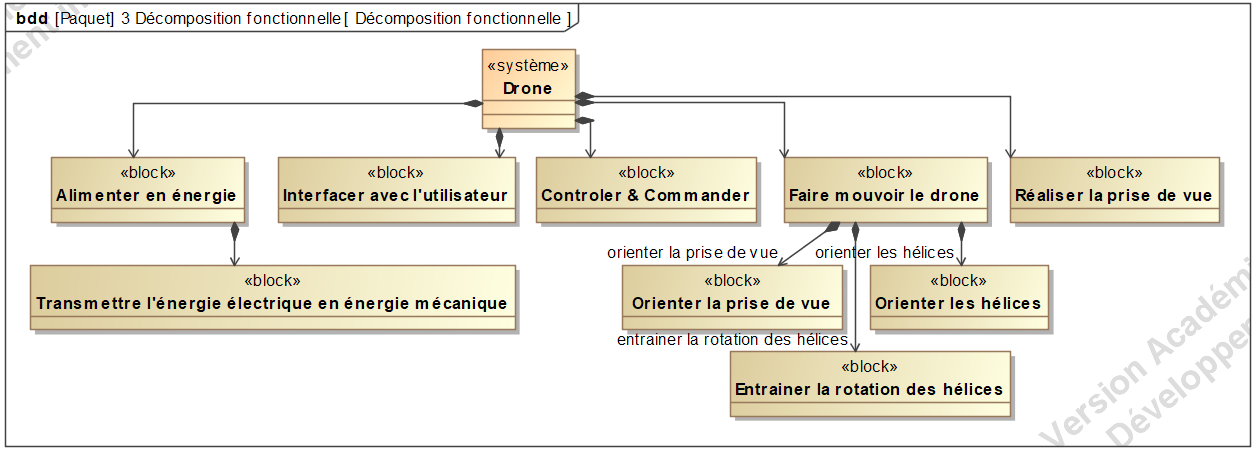
\includegraphics[width=\linewidth]{images/image56.png}

\paragraph*{Définir les interfaces fonctionnelles -
IBD}\label{duxe9finir-les-interfaces-fonctionnelles---ibd}
\addcontentsline{toc}{paragraph}{Définir les interfaces fonctionnelles -
IBD}

Après avoir déterminer les différentes fonctions, il est possible de
définir comment les flux transitent d'une fonction à l'autre. Ces flux
peuvent être de matière, d'énergie ou d'information.

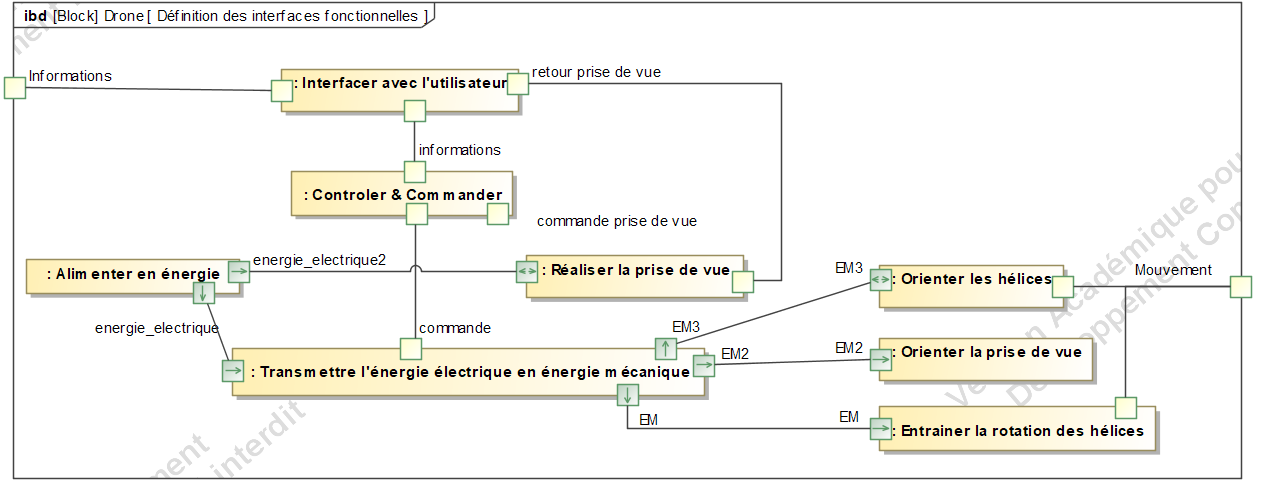
\includegraphics[width=\linewidth]{images/image57.png}

Cette architecture fonctionnelle va permettre de chercher des composants
existants permettant de réaliser cette fonction ou d'en créer des
nouveaux, ce qui sera l'intérêt de l'activité suivante. De plus, par les
interfaces, il est possible d'avoir des critères de fonctionnement.

\section{\texorpdfstring{Architecture fonctionnelle et chaines
fonctionnelles
}{Architecture fonctionnelle et chaines fonctionnelles }}\label{architecture-fonctionnelle-et-chaines-fonctionnelles}

Les systèmes pluri-techniques complexes, en particulier ceux qui sont
automatisés, peuvent être décrits à l'aide d'une architecture
fonctionnelle qui fait apparaitre :

\begin{itemize}
\item
  des blocs qui correspondent aux \textbf{Fonctions Techniques
  génériques} du système~;
\item
  les \textbf{flux d'énergie et d'information} qui circulent entre ces
  blocs.
\end{itemize}

Une fois que le cahier des charges fonctionnel est bien défini, il est
important de définir quelles seront les fonctions qui vont y répondre.
Afin de faciliter la conception des systèmes, plusieurs patrons de
conception existent dont celui de la \textbf{chaine d'information et de
la chaine de puissance} (instantanée).

Energie électrique DC modulée

Energie électrique AC modulée

Energie pneumatique modulée

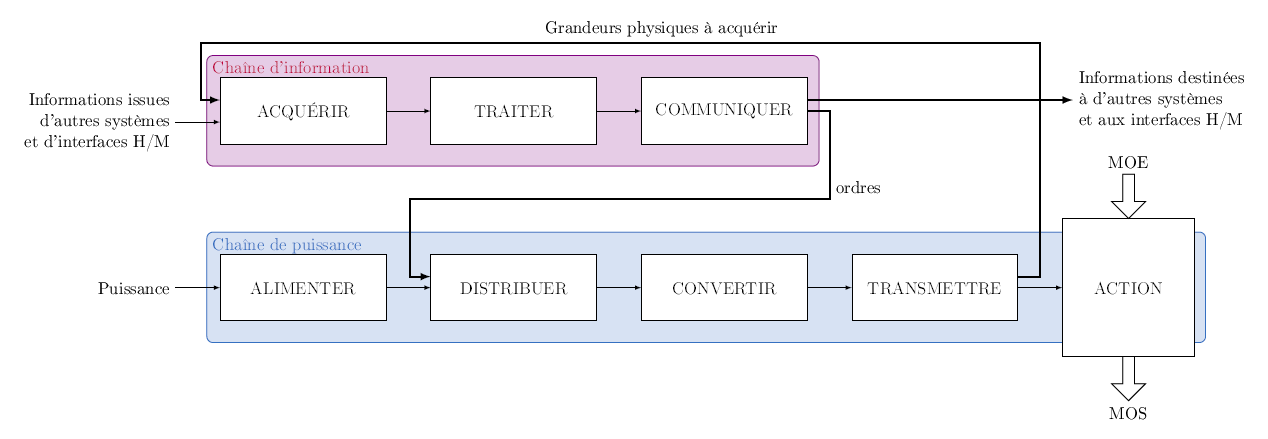
\includegraphics[width=\linewidth]{images/image58.png}

Energie mécanique de rotation

Energie mécanique de translation

Hacheur

Onduleur

Onduleur

Distributeur

Energie électrique DC

Energie électrique AC

Energie électrique DC

MCC

MAS

MS

vérin

Remarque~: parfois DISTRIBUER est remplacé par MODULER, on trouve aussi
parfois CODER entre ACQUERIR et TRAITER

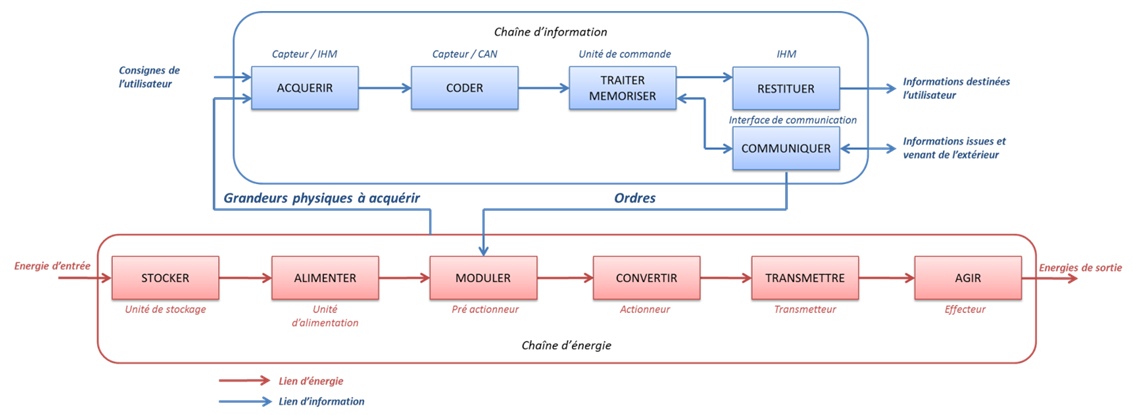
\includegraphics[width=\linewidth]{images/image59.png}

\textbf{Lien d'information :} Un lien d'information véhicule une
information. Très souvent, la nature su signal est de type électrique
(en \emph{V}).

\textbf{Lien de puissance (ou d'énergie) :} Un lien de puissance
véhicule une grandeur de type \textbf{effort} et une grandeur de type
\textbf{flux}. Le produit de ces deux grandeurs est une puissance.

\begin{longtable}[]{@{}
  >{\raggedright\arraybackslash}p{(\columnwidth - 4\tabcolsep) * \real{0.3240}}
  >{\raggedright\arraybackslash}p{(\columnwidth - 4\tabcolsep) * \real{0.3174}}
  >{\raggedright\arraybackslash}p{(\columnwidth - 4\tabcolsep) * \real{0.3586}}@{}}
\toprule\noalign{}
\begin{minipage}[b]{\linewidth}\raggedright
\textbf{Domaine}
\end{minipage} & \begin{minipage}[b]{\linewidth}\raggedright
\textbf{Effort}
\end{minipage} & \begin{minipage}[b]{\linewidth}\raggedright
\textbf{Flux}
\end{minipage} \\
\midrule\noalign{}
\endhead
\bottomrule\noalign{}
\endlastfoot
Électrotechnique & Tension (\emph{U} en \emph{V}) & Courant (\emph{I} en
\emph{A}) \\
Mécanique de translation & Force (\emph{F} en \emph{N}) & Vitesse
(\emph{V} en \emph{m/s}) \\
Mécanique de rotation & Couple (\emph{C} en \emph{N.m}) & Vitesse de
rotation (en \emph{rad /s}) \\
Hydraulique -- Pneumatique & Pression (\emph{P} en \emph{Pa}) & Débit
volumique (\emph{q} en \emph{m\textsuperscript{3}/s}) \\
\end{longtable}



\begin{exercice}{Exercice 1 -- Analyse fonctionnelle}

\begin{enumerate}
\def\labelenumi{\arabic{enumi}.}
\item
  Réaliser les chaines fonctionnelles d'un four électrique.
\item
  Réaliser les chaines fonctionnelles du drone.
\end{enumerate}

\vspace{5cm}

\end{exercice}

\begin{longtable}[]{@{}
  >{\raggedright\arraybackslash}p{(\columnwidth - 2\tabcolsep) * \real{0.1227}}
  >{\raggedright\arraybackslash}p{(\columnwidth - 2\tabcolsep) * \real{0.8773}}@{}}
\toprule\noalign{}
\begin{minipage}[b]{\linewidth}\raggedright
\begin{quote}

\includegraphics[width=\linewidth]{images/image52.png}
\end{quote}
\end{minipage} & \begin{minipage}[b]{\linewidth}\raggedright
\begin{enumerate}
\def\labelenumi{\arabic{enumi}.}
\item
  Réaliser les chaines fonctionnelles d'un four électrique.
\item
  Réaliser les chaines fonctionnelles du drone.
\end{enumerate}
\end{minipage} \\
\midrule\noalign{}
\endhead
\bottomrule\noalign{}
\endlastfoot
\end{longtable}

\section{Sources}\label{sources}

Ce cours a été élaboré à l'aide de nombreuses ressources~:

\begin{itemize}
\item
  Les standards d'ingénierie Système~: ISO 15288, EIA 632, SEBoK et
  autres documents de l'AFIS (Association Française de l'Ingénierie
  Système)
\item
  Des documents publics d'industriels~: PSA, Thalès, Schneider Electric
\item
  Des activités pédagogiques de collègues de l'UPSTI, Yan Le Gallou,
  Pierre Mauborgne
\end{itemize}

\subsection{Principaux constituants}\label{principaux-constituants}

\begin{longtable}[]{@{}
  >{\raggedright\arraybackslash}p{(\columnwidth - 18\tabcolsep) * \real{0.0104}}
  >{\raggedright\arraybackslash}p{(\columnwidth - 18\tabcolsep) * \real{0.1867}}
  >{\raggedright\arraybackslash}p{(\columnwidth - 18\tabcolsep) * \real{0.0311}}
  >{\raggedright\arraybackslash}p{(\columnwidth - 18\tabcolsep) * \real{0.0104}}
  >{\raggedright\arraybackslash}p{(\columnwidth - 18\tabcolsep) * \real{0.0415}}
  >{\raggedright\arraybackslash}p{(\columnwidth - 18\tabcolsep) * \real{0.3329}}
  >{\raggedright\arraybackslash}p{(\columnwidth - 18\tabcolsep) * \real{0.0133}}
  >{\raggedright\arraybackslash}p{(\columnwidth - 18\tabcolsep) * \real{0.0134}}
  >{\raggedright\arraybackslash}p{(\columnwidth - 18\tabcolsep) * \real{0.0102}}
  >{\raggedright\arraybackslash}p{(\columnwidth - 18\tabcolsep) * \real{0.3502}}@{}}
\toprule\noalign{}
\multicolumn{2}{@{}>{\raggedright\arraybackslash}p{(\columnwidth - 18\tabcolsep) * \real{0.1970} + 2\tabcolsep}}{%
\multirow{2}{=}{\begin{minipage}[b]{\linewidth}\raggedright
\begin{quote}
\textbf{Pré-actionneur}
\end{quote}
\end{minipage}}} &
\multicolumn{7}{>{\raggedright\arraybackslash}p{(\columnwidth - 18\tabcolsep) * \real{0.4527} + 12\tabcolsep}}{%
\begin{minipage}[b]{\linewidth}\raggedright
\emph{\textbf{Fonction}}
\end{minipage}} &
\multirow{2}{=}{\begin{minipage}[b]{\linewidth}\raggedright
\begin{quote}
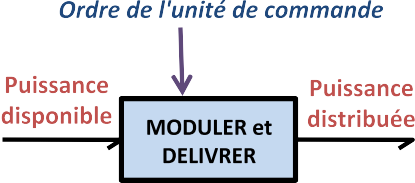
\includegraphics[width=\linewidth]{images/image60.png}


\includegraphics[width=0.81806in,height=\textheight]{images/image61.png}
\end{quote}
\end{minipage}} \\
& &
\multicolumn{7}{>{\raggedright\arraybackslash}p{(\columnwidth - 18\tabcolsep) * \real{0.4527} + 12\tabcolsep}}{%
\begin{minipage}[b]{\linewidth}\raggedright
\begin{quote}
\emph{Délivrer, sur ordre de l'unité de commande, la puissance utile aux
actionneurs.}
\end{quote}
\end{minipage}} \\
\midrule\noalign{}
\endhead
\bottomrule\noalign{}
\endlastfoot
\multicolumn{10}{@{}>{\raggedright\arraybackslash}p{(\columnwidth - 18\tabcolsep) * \real{1.0000} + 18\tabcolsep}@{}}{%
\begin{minipage}[t]{\linewidth}\raggedright
\begin{quote}
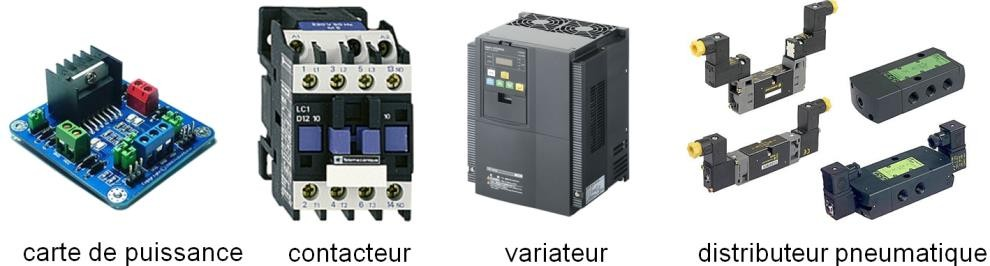
\includegraphics[width=\linewidth]{images/image62.jpeg}
\end{quote}
\end{minipage}} \\
\multicolumn{3}{@{}>{\raggedright\arraybackslash}p{(\columnwidth - 18\tabcolsep) * \real{0.2282} + 4\tabcolsep}}{%
\multirow{2}{=}{\begin{minipage}[t]{\linewidth}\raggedright
\begin{quote}
\textbf{Actionneur}
\end{quote}
\end{minipage}}} &
\multicolumn{4}{>{\raggedright\arraybackslash}p{(\columnwidth - 18\tabcolsep) * \real{0.3980} + 6\tabcolsep}}{%
\emph{\textbf{Fonction}}} &
\multicolumn{3}{>{\raggedright\arraybackslash}p{(\columnwidth - 18\tabcolsep) * \real{0.3738} + 4\tabcolsep}@{}}{%
\multirow{2}{=}{\begin{minipage}[t]{\linewidth}\raggedright
\begin{quote}
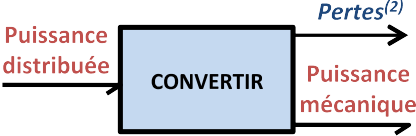
\includegraphics[width=\linewidth]{images/image63.png}


\includegraphics[width=0.61042in,height=\textheight]{images/image64.png}
\end{quote}
\end{minipage}}} \\
& & &
\multicolumn{4}{>{\raggedright\arraybackslash}p{(\columnwidth - 18\tabcolsep) * \real{0.3980} + 6\tabcolsep}}{%
\begin{minipage}[t]{\linewidth}\raggedright
\begin{quote}
\emph{Convertir la puissance distribuée en puissance mécanique (de
translation ou de rotation)}.
\end{quote}
\end{minipage}} \\
\multicolumn{10}{@{}>{\raggedright\arraybackslash}p{(\columnwidth - 18\tabcolsep) * \real{1.0000} + 18\tabcolsep}@{}}{%
\begin{minipage}[t]{\linewidth}\raggedright
\begin{quote}
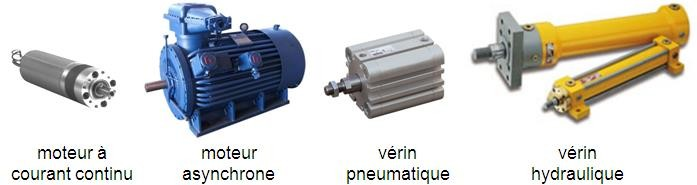
\includegraphics[width=\linewidth]{images/image65.jpeg}
\end{quote}
\end{minipage}} \\
\multicolumn{3}{@{}>{\raggedright\arraybackslash}p{(\columnwidth - 18\tabcolsep) * \real{0.2282} + 4\tabcolsep}}{%
\multirow{2}{=}{\begin{minipage}[t]{\linewidth}\raggedright
\begin{quote}
\textbf{Transmetteur}
\end{quote}
\end{minipage}}} &
\multicolumn{3}{>{\raggedright\arraybackslash}p{(\columnwidth - 18\tabcolsep) * \real{0.3847} + 4\tabcolsep}}{%
\emph{\textbf{Fonction}}} &
\multicolumn{4}{>{\raggedright\arraybackslash}p{(\columnwidth - 18\tabcolsep) * \real{0.3871} + 6\tabcolsep}@{}}{%
\multirow{2}{=}{\begin{minipage}[t]{\linewidth}\raggedright
\begin{quote}
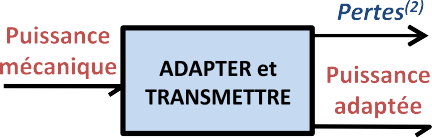
\includegraphics[width=\linewidth]{images/image66.png}


\includegraphics[width=0.75347in,height=\textheight]{images/image67.png}
\end{quote}
\end{minipage}}} \\
& & &
\multicolumn{3}{>{\raggedright\arraybackslash}p{(\columnwidth - 18\tabcolsep) * \real{0.3847} + 4\tabcolsep}}{%
\begin{minipage}[t]{\linewidth}\raggedright
\begin{quote}
\emph{Adapter et transmettre la puissance mécanique délivrée par
l'actionneur pour la rendre utilisable par l'effecteur.}
\end{quote}
\end{minipage}} \\
\multicolumn{6}{@{}>{\raggedright\arraybackslash}p{(\columnwidth - 18\tabcolsep) * \real{0.6129} + 10\tabcolsep}}{%
\begin{minipage}[t]{\linewidth}\raggedright
\begin{quote}
Sans transformation de mouvement
\end{quote}
\end{minipage}} &
\multicolumn{4}{>{\raggedright\arraybackslash}p{(\columnwidth - 18\tabcolsep) * \real{0.3871} + 6\tabcolsep}@{}}{%
Avec transformation du mouvement} \\
\multicolumn{6}{@{}>{\raggedright\arraybackslash}p{(\columnwidth - 18\tabcolsep) * \real{0.6129} + 10\tabcolsep}}{%
\begin{minipage}[t]{\linewidth}\raggedright
\begin{quote}
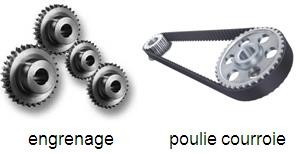
\includegraphics[width=\linewidth]{images/image68.jpeg}
\end{quote}
\end{minipage}} &
\multicolumn{4}{>{\raggedright\arraybackslash}p{(\columnwidth - 18\tabcolsep) * \real{0.3871} + 6\tabcolsep}@{}}{%
\begin{minipage}[t]{\linewidth}\raggedright
\begin{quote}
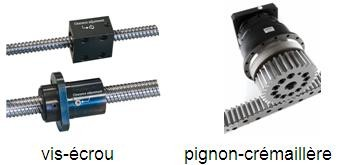
\includegraphics[width=\linewidth]{images/image69.jpeg}
\end{quote}
\end{minipage}} \\
\multicolumn{2}{@{}>{\raggedright\arraybackslash}p{(\columnwidth - 18\tabcolsep) * \real{0.1970} + 2\tabcolsep}}{%
\multirow{2}{=}{\begin{minipage}[t]{\linewidth}\raggedright
\begin{quote}
\textbf{Effecteur}
\end{quote}
\end{minipage}}} &
\multicolumn{7}{>{\raggedright\arraybackslash}p{(\columnwidth - 18\tabcolsep) * \real{0.4527} + 12\tabcolsep}}{%
\emph{\textbf{Fonction}}} &
\multirow{2}{=}{\begin{minipage}[t]{\linewidth}\raggedright
\begin{quote}
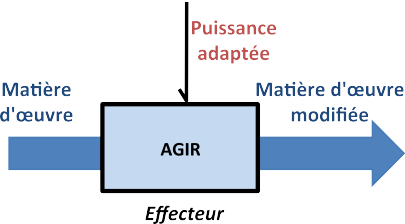
\includegraphics[width=\linewidth]{images/image70.png}
\end{quote}
\end{minipage}} \\
& &
\multicolumn{7}{>{\raggedright\arraybackslash}p{(\columnwidth - 18\tabcolsep) * \real{0.4527} + 12\tabcolsep}}{%
\begin{minipage}[t]{\linewidth}\raggedright
\begin{quote}
\emph{Effectuer la transformation de la matière d'œuvre.}

\emph{\ul{Exemples:} doigts d'une pince, tapis roulant, outil d'un
centre d'usinage, ventouse ou électro-aimant d'un système de
préhension\ldots{}}
\end{quote}
\end{minipage}} \\
\multicolumn{3}{@{}>{\raggedright\arraybackslash}p{(\columnwidth - 18\tabcolsep) * \real{0.2282} + 4\tabcolsep}}{%
\multirow{2}{=}{\begin{minipage}[t]{\linewidth}\raggedright
\begin{quote}
\textbf{Capteur}
\end{quote}
\end{minipage}}} &
\multicolumn{5}{>{\raggedright\arraybackslash}p{(\columnwidth - 18\tabcolsep) * \real{0.4114} + 8\tabcolsep}}{%
\emph{\textbf{Fonction}}} &
\multirow{2}{=}{\begin{minipage}[t]{\linewidth}\raggedright
\begin{quote}
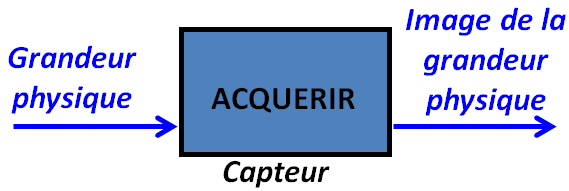
\includegraphics[width=\linewidth]{images/image71.png}
\end{quote}
\end{minipage}} & \\
& & &
\multicolumn{5}{>{\raggedright\arraybackslash}p{(\columnwidth - 18\tabcolsep) * \real{0.4114} + 8\tabcolsep}}{%
\begin{minipage}[t]{\linewidth}\raggedright
\begin{quote}
\emph{Prélever une grandeur physique et en produire une image
exploitable par l'unité de commande.}
\end{quote}
\end{minipage}} & & \\
\multicolumn{9}{@{}>{\raggedright\arraybackslash}p{(\columnwidth - 18\tabcolsep) * \real{0.6498} + 16\tabcolsep}}{%
\begin{minipage}[t]{\linewidth}\raggedright
\begin{quote}
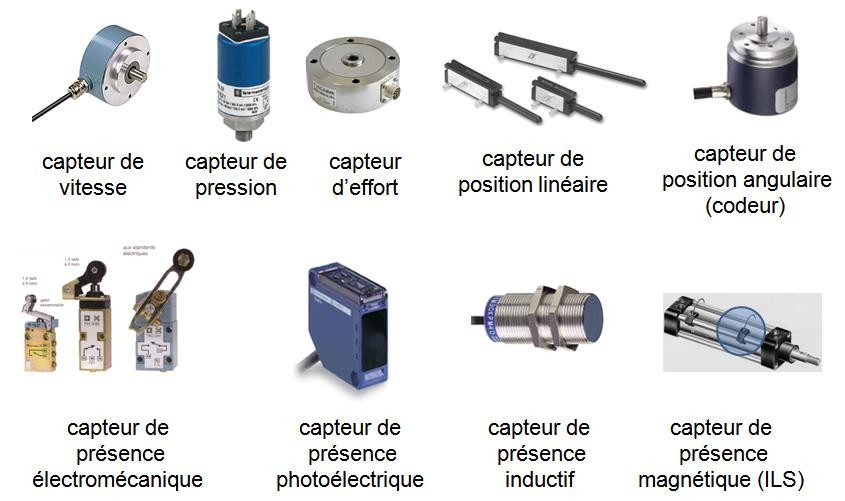
\includegraphics[width=\linewidth]{images/image72.jpeg}

\emph{Et aussi : capteur d'accélération, capteur de température\ldots{}}
\end{quote}
\end{minipage}} & \\
\multicolumn{4}{@{}>{\raggedright\arraybackslash}p{(\columnwidth - 18\tabcolsep) * \real{0.2385} + 6\tabcolsep}}{%
\multirow{3}{=}{\begin{minipage}[t]{\linewidth}\raggedright
\begin{quote}
\textbf{Interface Homme/Machine}
\end{quote}
\end{minipage}}} &
\multicolumn{3}{>{\raggedright\arraybackslash}p{(\columnwidth - 18\tabcolsep) * \real{0.3877} + 4\tabcolsep}}{%
\begin{minipage}[t]{\linewidth}\raggedright
\begin{quote}
\emph{\textbf{Fonctions}}
\end{quote}
\end{minipage}} &
\multicolumn{2}{>{\raggedright\arraybackslash}p{(\columnwidth - 18\tabcolsep) * \real{0.0236} + 2\tabcolsep}}{%
\multirow{2}{=}{\begin{minipage}[t]{\linewidth}\raggedright
\begin{quote}
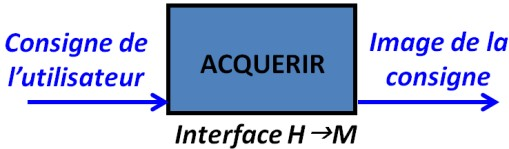
\includegraphics[width=\linewidth]{images/image73.jpeg}
\end{quote}
\end{minipage}}} & \\
& & & &
\multicolumn{3}{>{\raggedright\arraybackslash}p{(\columnwidth - 18\tabcolsep) * \real{0.3877} + 4\tabcolsep}}{%
\begin{minipage}[t]{\linewidth}\raggedright
\begin{quote}
\emph{Traduire la consigne d'un utilisateur en une image exploitable par
la partie commande.}
\end{quote}
\end{minipage}} & & & \\
& & & &
\multicolumn{3}{>{\raggedright\arraybackslash}p{(\columnwidth - 18\tabcolsep) * \real{0.3877} + 4\tabcolsep}}{%
\begin{minipage}[t]{\linewidth}\raggedright
\begin{quote}
\emph{Permettre à l'utilisateur d'être informé sur l'état du système.}
\end{quote}
\end{minipage}} &
\multicolumn{2}{>{\raggedright\arraybackslash}p{(\columnwidth - 18\tabcolsep) * \real{0.0236} + 2\tabcolsep}}{%
\begin{minipage}[t]{\linewidth}\raggedright
\begin{quote}
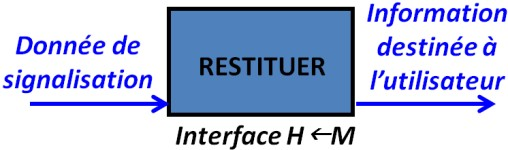
\includegraphics[width=\linewidth]{images/image74.jpeg}
\end{quote}
\end{minipage}} & \\
\multicolumn{9}{@{}>{\raggedright\arraybackslash}p{(\columnwidth - 18\tabcolsep) * \real{0.6498} + 16\tabcolsep}}{%
\begin{minipage}[t]{\linewidth}\raggedright
\begin{quote}
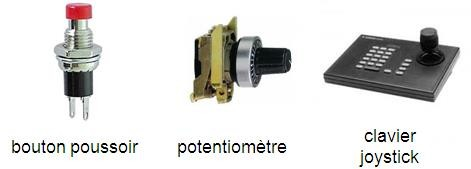
\includegraphics[width=\linewidth]{images/image75.jpeg}
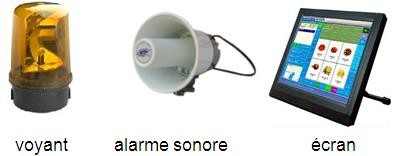
\includegraphics[width=\linewidth]{images/image76.jpeg}

\emph{Et aussi : bouton coup de poing, interrupteur de position, écran
tactile\ldots{}}
\end{quote}
\end{minipage}} & \\
\end{longtable}

\begin{longtable}[]{@{}
  >{\raggedright\arraybackslash}p{(\columnwidth - 8\tabcolsep) * \real{0.1355}}
  >{\raggedright\arraybackslash}p{(\columnwidth - 8\tabcolsep) * \real{0.0541}}
  >{\raggedright\arraybackslash}p{(\columnwidth - 8\tabcolsep) * \real{0.1894}}
  >{\raggedright\arraybackslash}p{(\columnwidth - 8\tabcolsep) * \real{0.2221}}
  >{\raggedright\arraybackslash}p{(\columnwidth - 8\tabcolsep) * \real{0.3989}}@{}}
\toprule\noalign{}
\multirow{2}{=}{\begin{minipage}[b]{\linewidth}\raggedright
\begin{quote}
\textbf{Unité de Commande}
\end{quote}
\end{minipage}} &
\multicolumn{3}{>{\raggedright\arraybackslash}p{(\columnwidth - 8\tabcolsep) * \real{0.4656} + 4\tabcolsep}}{%
\begin{minipage}[b]{\linewidth}\raggedright
\emph{\textbf{Fonction}}
\end{minipage}} &
\multirow{2}{=}{\begin{minipage}[b]{\linewidth}\raggedright
\begin{quote}
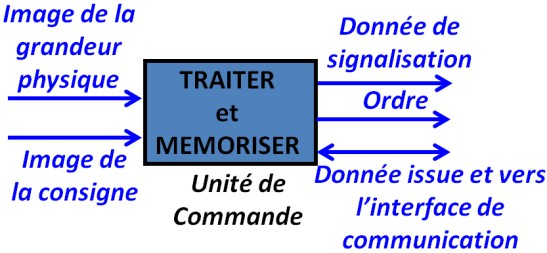
\includegraphics[width=\linewidth]{images/image77.jpeg}
\end{quote}
\end{minipage}} \\
&
\multicolumn{3}{>{\raggedright\arraybackslash}p{(\columnwidth - 8\tabcolsep) * \real{0.4656} + 4\tabcolsep}}{%
\begin{minipage}[b]{\linewidth}\raggedright
\begin{quote}
\emph{Traiter, à l'aide du programme implanté en mémoire, les
informations en provenance des capteurs et de l'interface H $\rightarrow$ M afin
d'émettre les ordres destinés aux pré-actionneurs des différentes
chaines d'énergie du système.}

\emph{Envoyer des signalisations à l'interface M $\rightarrow$ H qui seront traduites
en messages écrits ou en signaux lumineux et/ou sonores à destination de
l'utilisateur.}
\end{quote}
\end{minipage}} \\
\midrule\noalign{}
\endhead
\bottomrule\noalign{}
\endlastfoot
\multicolumn{5}{@{}>{\raggedright\arraybackslash}p{(\columnwidth - 8\tabcolsep) * \real{1.0000} + 8\tabcolsep}@{}}{%
\begin{minipage}[t]{\linewidth}\raggedright
\begin{quote}
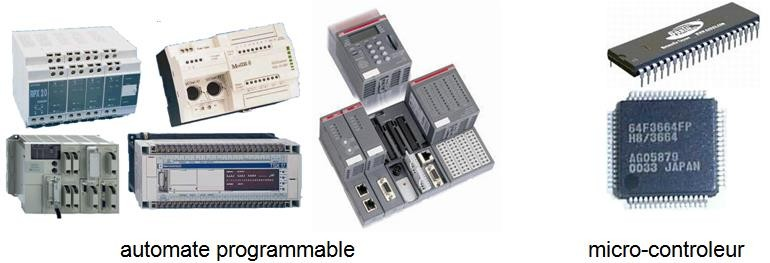
\includegraphics[width=\linewidth]{images/image78.jpeg}
\end{quote}
\end{minipage}} \\
\multicolumn{2}{@{}>{\raggedright\arraybackslash}p{(\columnwidth - 8\tabcolsep) * \real{0.1896} + 2\tabcolsep}}{%
\multirow{2}{=}{\begin{minipage}[t]{\linewidth}\raggedright
\begin{quote}
\textbf{Interface de communication}
\end{quote}
\end{minipage}}} & \begin{minipage}[t]{\linewidth}\raggedright
\begin{quote}
\emph{\textbf{Fonction}}
\end{quote}
\end{minipage} &
\multicolumn{2}{>{\raggedright\arraybackslash}p{(\columnwidth - 8\tabcolsep) * \real{0.6210} + 2\tabcolsep}@{}}{%
\multirow{2}{=}{\begin{minipage}[t]{\linewidth}\raggedright
\begin{quote}
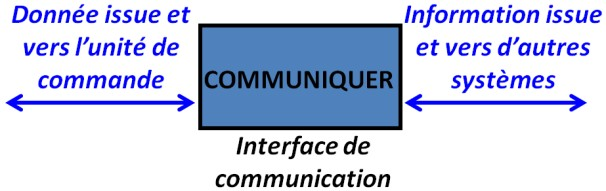
\includegraphics[width=\linewidth]{images/image79.jpeg}
\end{quote}
\end{minipage}}} \\
& & \begin{minipage}[t]{\linewidth}\raggedright
\begin{quote}
\emph{Permettre au système d'échanger des informations avec
l'extérieur.}
\end{quote}
\end{minipage} \\
\multicolumn{5}{@{}>{\raggedright\arraybackslash}p{(\columnwidth - 8\tabcolsep) * \real{1.0000} + 8\tabcolsep}@{}}{%
\begin{minipage}[t]{\linewidth}\raggedright
\begin{quote}
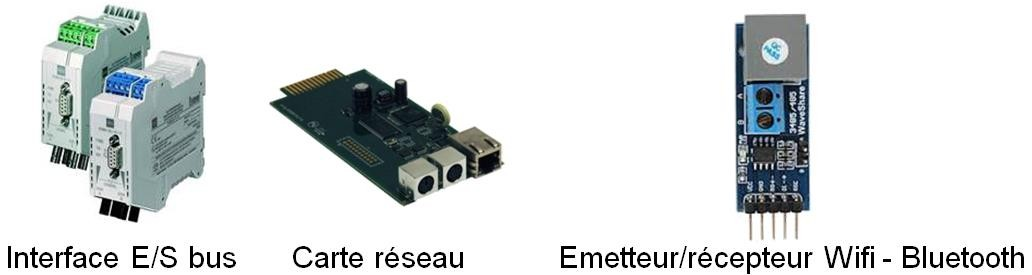
\includegraphics[width=\linewidth]{images/image80.jpeg}
\end{quote}
\end{minipage}} \\
\end{longtable}

\begin{enumerate}
\def\labelenumi{\arabic{enumi}.}
\item
  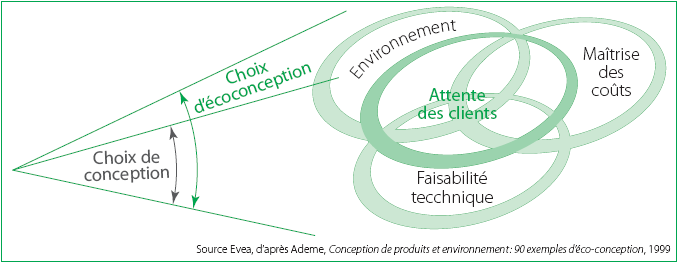
\includegraphics[width=\linewidth]{images/image81.png}Notions
  d'éco-conception
\end{enumerate}

Avec l'éco-conception, on sort de l'habituelle vision des industriels
qui ne prend en compte l'environnement que sur le site de production.

«~Eco-concevoir~», c'est dès la conception, essayer de \textbf{réduire
l'impact} \textbf{environnemental} que va avoir un système à toutes
\textbf{les étapes de son cycle de vie}, depuis l'extraction des
matières premières jusqu'à son traitement en fin de vie.

 $\rightarrow$  \textbf{\ul{Pourquoi éco-concevoir}}

La production de biens et de services contribue, de façon significative,
aux impacts environnementaux :

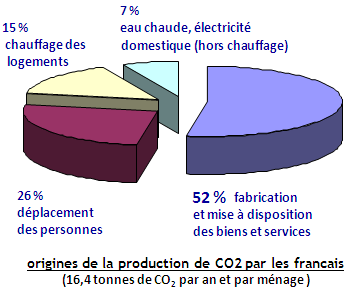
\includegraphics[width=0.5\linewidth]{images/image82.png}
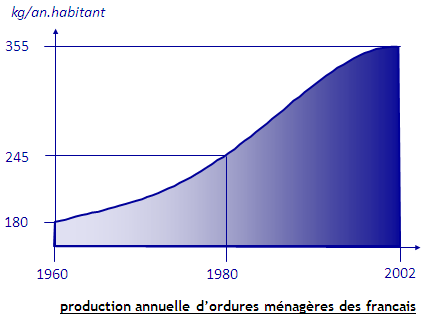
\includegraphics[width=0.5\linewidth]{images/image83.png}

Avec les 9 millions d'habitants qui peupleront la planète en 2040 et le
confort auquel ils aspirent, ces impacts doivent être impérativement
limités afin de tendre vers un mode de vie durable pour tous.

Mais il existe d'autres raisons qui poussent les entreprises à
éco-concevoir~:

\begin{itemize}
\item
  la recherche de la compétitivité avec l'apparition de nouveaux
  marchés~en utilisant l'éco-conception comme levier pour l'innovation ;
\item
  les pressions externes (réglementation, normes\ldots) et les attentes
  des clients (boycott, labels\ldots)~;
\item
  la diminution des coûts (recyclage des matières, réduction des
  emballages, diminution des coûts de dépollution\ldots).
\end{itemize}




\end{document}
